% !TeX root = RJwrapper.tex
\title{Lending Environment Simulator and Lender Evaluation Tool}
\author{by Vadim Spirkov, Murlidhar Loka}

\maketitle

\abstract{%
In the world of financial credit the industry practitioners are
topically confronted by the following questions:

\begin{itemize}
\item
  How strong are my potential business partners financially so my
  organization can create a long term relationship with them?
\item
  How much risk is involved in dealing with a particular person or a
  business so I could manage it better?
\end{itemize}

To answer such questions the credit industry has developed a few scoring
techniques to evaluate credit risk of a business or a person. These
scoring algorithms traditionally use historical financial data to
forecast a near-term outlook and a long-term viability scenario. In
recent years Machine-Learning software took the industry by storm
offering in-depth understanding of the valuable connections between
pieces of data. It is hard for human analysts alone to match the speed,
efficiency and accuracy of ML models, particularly in the
high-dimensional, large-volume data space.

This paper applies rather an unorthodox approach to a credit evaluation
problem. But before we proceed any further we would like to introduce
our business partner - KASI Insight. KASI Insights is an award-winning
and leading provider of consumer data, measures and insights to
understand average African consumer. Every month, the company listens to
Africans and turns survey based data into actionable insights. Through
its self-service platform, the clients of the firm leverage consumer
insights at scale, identify early signs of market shifts and unlock
market-creating opportunities for their businesses. (Ref:\cite{kasi})

One of the groups KASI Insight surveys are people who actively lend
money to other community members. In Africa money lending between the
individuals is very common and popular. This practice, in fact, is a
substitution to the small loan franchises, which are wide-spread in
Western countries. The firm leverages the wisdom of the crowd to
evaluate lending activities within a community over time to compute a
community-based score. Thus KASI's surveys provide risk profile of the
population in a given area through the eyes of the lender. KASI Insight
team was very interested in finding out:

\begin{itemize}
\item
  If the collected data could be translated into an individual credit
  score.
\item
  Whether there are any other applications of the collected data
  possible.
\item
  What useful or even commercially successful products could be created
  based on the available data.
\end{itemize}

Learning the business model of the company, the data it possesses we
have quickly realized that the traditional approach to the credit score
evaluation will not work in this particular case; KASI Insight does not
own financial data\ldots{} So we asked ourselves:

\begin{itemize}
\item
  How can we apply the survey data collected by KASI Insight over years
  to evaluate credit score of the community members?
\item
  Could the data be used to create other valuable products?
\item
  How can we employ Machine Learning techniques to produce a valuable
  content for KASI Insight?
\end{itemize}

This paper addresses all those questions. It provides in-depth analysis
of the survey data, explains its deficiency and offer means to fix the
data problems. In close collaboration with KASI Insight team, we design
two Machine-Learning based products that, we hope, will extend KASI
Insight offering to its business partners. They are:

\begin{itemize}
\item
  Lending Environment Simulator
\item
  Lender Evaluator
\end{itemize}

The paper walks the reader through the product design process, justifies
each solution, evaluates the results. In the end we provide a brief
overview of the turn-key solution we developed for KASI Insight.
}

% Any extra LaTeX you need in the preamble

\hypertarget{background}{%
\section{Background}\label{background}}

Let's briefly review how KASI Insight collects and uses the data.

\begin{itemize}
\item
  Samples from the community who have lent money (lenders) are pooled
  and asked questions about borrowers within the community based on
  their personal experience.
\item
  The responses to the survey are inputted into KASI Insight credit
  model and a community score is computed. The score is assigned to all
  members of the community.
\end{itemize}

After initial assessment of the process and the data we understood that
the existing approach was not suitable for Machine-Learning application.
We brainstormed and suggested two ways to utilize the available data.

Firstly we put ourselves in the shoes of a lender. Being a lender we
would be interested to know how our lending pattern would affect our
profit. For example if we start lending money to the business colleges
instead of family. Or what if we increase the interest, or we decrease
the interest and increase the amount or lending term, etc. Another use
case we considered was if we were a banker who were contemplating to
establish a quick loan business in a specific area how would we
evaluate, at least initially the credit worthiness of the population?
This is how we came up with the \textbf{Lending Environment Simulator}
concept. This ML model could be trained on the survey answers to assign
a credit category. To implement such a model we would have to have the
labels for all observations; we did not have them. We discussed the
problem with KASI Insight team. Our business partner came up with the
credit category formula, which is described below.

\hypertarget{credit-category-assignment-process}{%
\subsection{Credit Category Assignment
Process}\label{credit-category-assignment-process}}

KASI team assigned weights to the survey answers that pertain to the
lending practice. Based on the answers of each observation we calculated
the score, which was used to assign one of the five categories as
follows:

\begin{itemize}
\tightlist
\item
  \textbf{Very Poor} - the credit score less than \textbf{350}
\item
  \textbf{Poor} - the credit score is between \textbf{350 and 550}
\item
  \textbf{Fair} - the credit score is between \textbf{550 and 650}
\item
  \textbf{Good} - the credit score lies between \textbf{650 and 750}
\item
  \textbf{Very Good} - the credit score is higher than \textbf{750}
\end{itemize}

and this is how we labeled all observation to train the simulator
classifier.

\hypertarget{lender-evaluator}{%
\subsection{Lender Evaluator}\label{lender-evaluator}}

How else could we possibly use the data our business partner collected?
We though if we were a financial institution and wanted to have a proxy
to conduct money lending business in our behalf in various communities
how would we evaluate the business savviness of the potential
candidates? This is how we came up with the concept of \textbf{Lender
Evaluator} model.

We believed that the survey KASI Insight conducts not only reflect the
credit worthiness of the general public but also describe the
proficiency, knowledge and experience of the lender as a business
partner. We only needed the formula to evaluate the answers correctly in
this particular context. Again KASI Insight team was very instrumental.
They created another formula to calculate the lender score employing the
survey answers. We took similar to the simulator model approach. Only
the weights applied to the answers deferred. The categories for lenders
were identical to the credit categories listed above.

\hypertarget{objectives}{%
\section{Objectives}\label{objectives}}

Through exploring and applying the latest Machine-Learning techniques we
aim to deliver two ML models:

\begin{itemize}
\item
  Lending Environment Simulator
\item
  Lender Evaluator
\end{itemize}

We hope that these models will be included into the product line-up of
KASI Insight allowing our business partner to explore new business
opportunities. We will deliver the turn-key solution that would include
the user interface to demonstrate the model performance in real life.
The final product will also include a docker image to simplify the model
deployment into production environment on AWS cloud.

\hypertarget{project-artifacts}{%
\section{Project Artifacts}\label{project-artifacts}}

All project artifacts, technical guides, this report could be found at
\href{https://github.com/v2msLabs/ML1030-Capstone-Project}{GitHub}

\hypertarget{data-analysis}{%
\section{Data Analysis}\label{data-analysis}}

As it has been already stated we are dealing with the survey data
collected by KASI Insight from seven African countries. So far KASI
insight has collected almost \textbf{30,000} records over a course of
last three years.

\hypertarget{data-dictionary}{%
\subsection{Data Dictionary}\label{data-dictionary}}

The survey comprises 38 columns. Majority of them are multi-choice
questions. The table below lists the survey columns

\begin{longtable}[]{@{}ll@{}}
\toprule
\begin{minipage}[b]{0.05\columnwidth}\raggedright
ID\strut
\end{minipage} & \begin{minipage}[b]{0.89\columnwidth}\raggedright
Question/Column\strut
\end{minipage}\tabularnewline
\midrule
\endhead
\begin{minipage}[t]{0.05\columnwidth}\raggedright
0\strut
\end{minipage} & \begin{minipage}[t]{0.89\columnwidth}\raggedright
Timestamp\strut
\end{minipage}\tabularnewline
\begin{minipage}[t]{0.05\columnwidth}\raggedright
1\strut
\end{minipage} & \begin{minipage}[t]{0.89\columnwidth}\raggedright
Location ID\strut
\end{minipage}\tabularnewline
\begin{minipage}[t]{0.05\columnwidth}\raggedright
2\strut
\end{minipage} & \begin{minipage}[t]{0.89\columnwidth}\raggedright
Has it become more difficult or easier to find a job in your city?\strut
\end{minipage}\tabularnewline
\begin{minipage}[t]{0.05\columnwidth}\raggedright
3\strut
\end{minipage} & \begin{minipage}[t]{0.89\columnwidth}\raggedright
Is this a good time for people to make a large purchase such as
furniture or electrical appliances, given the economic climate?\strut
\end{minipage}\tabularnewline
\begin{minipage}[t]{0.05\columnwidth}\raggedright
4\strut
\end{minipage} & \begin{minipage}[t]{0.89\columnwidth}\raggedright
Compared to the last 6 months, are you able to spend (more, the same or
less) money on large purchases over the next 6 months?\strut
\end{minipage}\tabularnewline
\begin{minipage}[t]{0.05\columnwidth}\raggedright
5\strut
\end{minipage} & \begin{minipage}[t]{0.89\columnwidth}\raggedright
Will you be able to meet your regular expenses over the next 6
months?\strut
\end{minipage}\tabularnewline
\begin{minipage}[t]{0.05\columnwidth}\raggedright
6\strut
\end{minipage} & \begin{minipage}[t]{0.89\columnwidth}\raggedright
How do you expect your household's income to change over the next 6
months?\strut
\end{minipage}\tabularnewline
\begin{minipage}[t]{0.05\columnwidth}\raggedright
7\strut
\end{minipage} & \begin{minipage}[t]{0.89\columnwidth}\raggedright
How do you expect general economic conditions in your city to change
over the next 6 months?\strut
\end{minipage}\tabularnewline
\begin{minipage}[t]{0.05\columnwidth}\raggedright
8\strut
\end{minipage} & \begin{minipage}[t]{0.89\columnwidth}\raggedright
How do you expect general economic conditions in your country to change
over the next 6 months?\strut
\end{minipage}\tabularnewline
\begin{minipage}[t]{0.05\columnwidth}\raggedright
9\strut
\end{minipage} & \begin{minipage}[t]{0.89\columnwidth}\raggedright
Gender\strut
\end{minipage}\tabularnewline
\begin{minipage}[t]{0.05\columnwidth}\raggedright
10\strut
\end{minipage} & \begin{minipage}[t]{0.89\columnwidth}\raggedright
Marital status\strut
\end{minipage}\tabularnewline
\begin{minipage}[t]{0.05\columnwidth}\raggedright
11\strut
\end{minipage} & \begin{minipage}[t]{0.89\columnwidth}\raggedright
Age\strut
\end{minipage}\tabularnewline
\begin{minipage}[t]{0.05\columnwidth}\raggedright
12\strut
\end{minipage} & \begin{minipage}[t]{0.89\columnwidth}\raggedright
What's your highest level of education?\strut
\end{minipage}\tabularnewline
\begin{minipage}[t]{0.05\columnwidth}\raggedright
13\strut
\end{minipage} & \begin{minipage}[t]{0.89\columnwidth}\raggedright
Occupation\strut
\end{minipage}\tabularnewline
\begin{minipage}[t]{0.05\columnwidth}\raggedright
14\strut
\end{minipage} & \begin{minipage}[t]{0.89\columnwidth}\raggedright
If you are a student, what level are you currently studying?\strut
\end{minipage}\tabularnewline
\begin{minipage}[t]{0.05\columnwidth}\raggedright
15\strut
\end{minipage} & \begin{minipage}[t]{0.89\columnwidth}\raggedright
Race/Ethnicity\strut
\end{minipage}\tabularnewline
\begin{minipage}[t]{0.05\columnwidth}\raggedright
16\strut
\end{minipage} & \begin{minipage}[t]{0.89\columnwidth}\raggedright
Country\strut
\end{minipage}\tabularnewline
\begin{minipage}[t]{0.05\columnwidth}\raggedright
17\strut
\end{minipage} & \begin{minipage}[t]{0.89\columnwidth}\raggedright
What is the name of the neighborhood where you live?\strut
\end{minipage}\tabularnewline
\begin{minipage}[t]{0.05\columnwidth}\raggedright
18\strut
\end{minipage} & \begin{minipage}[t]{0.89\columnwidth}\raggedright
Over the past 3 months, how many times have you lent someone
money?\strut
\end{minipage}\tabularnewline
\begin{minipage}[t]{0.05\columnwidth}\raggedright
19\strut
\end{minipage} & \begin{minipage}[t]{0.89\columnwidth}\raggedright
On average how much do you lend in general?\strut
\end{minipage}\tabularnewline
\begin{minipage}[t]{0.05\columnwidth}\raggedright
20\strut
\end{minipage} & \begin{minipage}[t]{0.89\columnwidth}\raggedright
Who did you lend money to in the past 3 months?\strut
\end{minipage}\tabularnewline
\begin{minipage}[t]{0.05\columnwidth}\raggedright
21\strut
\end{minipage} & \begin{minipage}[t]{0.89\columnwidth}\raggedright
When you lend money, when do you usually expect to get it repaid?\strut
\end{minipage}\tabularnewline
\begin{minipage}[t]{0.05\columnwidth}\raggedright
22\strut
\end{minipage} & \begin{minipage}[t]{0.89\columnwidth}\raggedright
Do you include either interest or a lending fee when you lend?\strut
\end{minipage}\tabularnewline
\begin{minipage}[t]{0.05\columnwidth}\raggedright
23\strut
\end{minipage} & \begin{minipage}[t]{0.89\columnwidth}\raggedright
Do you request guarantees when you lend?\strut
\end{minipage}\tabularnewline
\begin{minipage}[t]{0.05\columnwidth}\raggedright
24\strut
\end{minipage} & \begin{minipage}[t]{0.89\columnwidth}\raggedright
Do you receive your money back in time?\strut
\end{minipage}\tabularnewline
\begin{minipage}[t]{0.05\columnwidth}\raggedright
25\strut
\end{minipage} & \begin{minipage}[t]{0.89\columnwidth}\raggedright
Assuming that you have lent money at least ten times, how often would
you get your money repaid?\strut
\end{minipage}\tabularnewline
\begin{minipage}[t]{0.05\columnwidth}\raggedright
26\strut
\end{minipage} & \begin{minipage}[t]{0.89\columnwidth}\raggedright
What's the most common use of the money you lend?\strut
\end{minipage}\tabularnewline
\begin{minipage}[t]{0.05\columnwidth}\raggedright
27\strut
\end{minipage} & \begin{minipage}[t]{0.89\columnwidth}\raggedright
Have you ever applied for a bank loan?\strut
\end{minipage}\tabularnewline
\begin{minipage}[t]{0.05\columnwidth}\raggedright
28\strut
\end{minipage} & \begin{minipage}[t]{0.89\columnwidth}\raggedright
Are you a tontine / lending club member?\strut
\end{minipage}\tabularnewline
\begin{minipage}[t]{0.05\columnwidth}\raggedright
29\strut
\end{minipage} & \begin{minipage}[t]{0.89\columnwidth}\raggedright
What is the most convenient way to get a loan?\strut
\end{minipage}\tabularnewline
\begin{minipage}[t]{0.05\columnwidth}\raggedright
30\strut
\end{minipage} & \begin{minipage}[t]{0.89\columnwidth}\raggedright
To what extent do you agree with the following sentences {[}Access to
credit is essential for me to achieve financial freedom{]}\strut
\end{minipage}\tabularnewline
\begin{minipage}[t]{0.05\columnwidth}\raggedright
31\strut
\end{minipage} & \begin{minipage}[t]{0.89\columnwidth}\raggedright
To what extent do you agree with the following sentences {[}Credit is
beneficial only if you have discipline{]}\strut
\end{minipage}\tabularnewline
\begin{minipage}[t]{0.05\columnwidth}\raggedright
32\strut
\end{minipage} & \begin{minipage}[t]{0.89\columnwidth}\raggedright
To what extent do you agree with the following sentences {[}I would like
to have more credit management training{]}\strut
\end{minipage}\tabularnewline
\begin{minipage}[t]{0.05\columnwidth}\raggedright
33\strut
\end{minipage} & \begin{minipage}[t]{0.89\columnwidth}\raggedright
What type of loans are you currently paying of?\strut
\end{minipage}\tabularnewline
\begin{minipage}[t]{0.05\columnwidth}\raggedright
34\strut
\end{minipage} & \begin{minipage}[t]{0.89\columnwidth}\raggedright
Do you have a credit score?\strut
\end{minipage}\tabularnewline
\begin{minipage}[t]{0.05\columnwidth}\raggedright
35\strut
\end{minipage} & \begin{minipage}[t]{0.89\columnwidth}\raggedright
Do you have a credit card?\strut
\end{minipage}\tabularnewline
\begin{minipage}[t]{0.05\columnwidth}\raggedright
36\strut
\end{minipage} & \begin{minipage}[t]{0.89\columnwidth}\raggedright
On average, how much of your total household monthly income do you spend
paying off debt each month?\strut
\end{minipage}\tabularnewline
\begin{minipage}[t]{0.05\columnwidth}\raggedright
37\strut
\end{minipage} & \begin{minipage}[t]{0.89\columnwidth}\raggedright
If you wanted to take a loan to start a business, how much would you
need?\strut
\end{minipage}\tabularnewline
\bottomrule
\end{longtable}

The survey data could be split into three major categories:

\begin{itemize}
\tightlist
\item
  Demographic Statistics.
\item
  Economic Sentiment.
\item
  Spending and Borrowing habits.
\end{itemize}

Each question/column should be treated as a categorical value.

\hypertarget{data-exploration}{%
\subsection{Data Exploration}\label{data-exploration}}

Let's take a look at the raw survey data (see the table below). Though
the survey multi-choice questions are categories in nature, the survey
answers are stored in alphanumeric format. Overtime some questions have
been rephrased. Thus in some cases the answers that pertain to the same
category vary. Another problem with the raw data set is the missing
values.

\begin{Schunk}
\begin{Soutput}
#>                             2                  3              4                  5
#> 0  Difficult / Plus difficile           No / Non    More / Plus  Maybe / Peut-être
#> 1  Difficult / Plus difficile           No / Non  Same / Pareil           No / Non
#> 2               Same / Pareil  Maybe / Peut-être  Same / Pareil  Maybe / Peut-être
#> 3               Same / Pareil           No / Non   Less / Moins           No / Non
#> 4               Same / Pareil           No / Non   Less / Moins  Maybe / Peut-être
\end{Soutput}
\begin{Soutput}
#>                          6                        7                        8               9
#> 0      Improve / Améliorée      Improve / Améliorée      Improve / Améliorée  Female / Femme
#> 1      Improve / Améliorée      Improve / Améliorée      Improve / Améliorée  Female / Femme
#> 2  Stay the same / La même  Stay the same / La même  Stay the same / La même    Male / Homme
#> 3      Worsen / Détériorée  Stay the same / La même  Stay the same / La même    Male / Homme
#> 4      Worsen / Détériorée  Stay the same / La même      Worsen / Détériorée    Male / Homme
\end{Soutput}
\begin{Soutput}
#>                                                   10     11                               12  \
#> 0  Separated, but not divorced / Séparé mais pas ...  18-24   High school, no diploma / BEPC   
#> 1                                 Dating / En couple  25-29      Bachelor’s degree / Licence   
#> 2                                    Married / Marié  18-24  Currently studying / Aux études   
#> 3                                    Married / Marié  40-44      Bachelor’s degree / Licence   
#> 4                                    Married / Marié  35-39      Bachelor’s degree / Licence   
#> 
#>                                                   13  
#> 0                        Salaried employee / Salarié  
#> 1                        Salaried employee / Salarié  
#> 2                           Unemployed / Sans emploi  
#> 3                        Business owner / Commercant  
#> 4  Commission-based employee / Employé sous commi...
\end{Soutput}
\end{Schunk}

To rectify the problems stated above we have developed a data processing
algorithm that normalized and categorized the answers converting them
into numeric form. The data processing script also imputes the missing
data with the most frequently occurring value for a given category. The
clean data set stats are depicted below. \textbf{Note}: the column
numbers correspond to the question numbers as described in \emph{Data
Dictionary} section

\begin{Schunk}
\begin{Soutput}
#>               2         3         4         5         6         7         8         9        10  \
#> count 29,383.00 29,383.00 29,383.00 29,383.00 29,383.00 29,383.00 29,383.00 29,383.00 29,383.00   
#> mean       1.69      2.07      1.90      2.16      1.80      1.82      1.83      1.66      1.99   
#> std        0.62      0.61      0.64      0.60      0.64      0.63      0.64      0.48      0.87   
#> min        1.00      1.00      1.00      1.00      1.00      1.00      1.00      1.00      1.00   
#> 25%        1.00      2.00      1.00      2.00      1.00      1.00      1.00      1.00      1.00   
#> 50%        2.00      2.00      2.00      2.00      2.00      2.00      2.00      2.00      2.00   
#> 75%        2.00      2.00      2.00      3.00      2.00      2.00      2.00      2.00      2.00   
#> max        3.00      3.00      3.00      3.00      3.00      3.00      3.00      2.00      7.00   
#> 
#>              11        12        13        14        16        18        19        20        21  \
#> count 29,383.00 29,383.00 29,383.00 29,383.00 29,383.00 29,383.00 29,383.00 29,383.00 29,383.00   
#> mean       3.68      3.85      2.77      0.24      3.59      2.41      2.07      1.93      2.39   
#> std        1.17      1.27      1.20      0.71      1.93      0.90      0.75      0.61      0.97   
#> min        1.00      1.00      1.00      0.00      1.00      1.00      1.00      1.00      1.00   
#> 25%        3.00      3.00      2.00      0.00      2.00      2.00      2.00      2.00      2.00   
#> 50%        4.00      4.00      3.00      0.00      4.00      2.00      2.00      2.00      2.00   
#> 75%        4.00      5.00      4.00      0.00      5.00      3.00      2.00      2.00      3.00   
#> max        9.00     10.00      9.00      4.00      7.00      4.00      4.00      3.00      6.00   
#> 
#>              22        23        24        25        26        27        28        29        30  \
#> count 29,383.00 29,383.00 29,383.00 29,383.00 29,383.00 29,383.00 29,383.00 29,383.00 29,383.00   
#> mean       3.26      3.28      2.80      2.71      2.61      1.47      1.51      2.66      2.71   
#> std        1.32      1.32      1.16      1.10      1.38      0.50      0.50      1.06      1.10   
#> min        1.00      1.00      1.00      1.00      1.00      1.00      1.00      1.00      1.00   
#> 25%        2.00      2.00      2.00      2.00      1.00      1.00      1.00      2.00      2.00   
#> 50%        3.00      3.00      3.00      3.00      2.00      1.00      2.00      2.00      2.00   
#> 75%        5.00      5.00      4.00      3.00      3.00      2.00      2.00      3.00      3.00   
#> max        5.00      5.00      5.00      5.00      5.00      2.00      2.00      6.00      5.00   
#> 
#>              31        32        33        34        35        36        37  credit_score  \
#> count 29,383.00 29,383.00 29,383.00 29,383.00 29,383.00 29,383.00 29,383.00     29,383.00   
#> mean       2.84      2.90      0.30      1.25      1.30      7.68      2.19        348.56   
#> std        1.13      1.22      1.08      0.44      0.46      1.26      0.58        244.70   
#> min        1.00      1.00      0.00      1.00      1.00      1.00      1.00       -720.00   
#> 25%        2.00      2.00      0.00      1.00      1.00      8.00      2.00        190.00   
#> 50%        2.00      2.00      0.00      1.00      1.00      8.00      2.00        390.00   
#> 75%        4.00      4.00      0.00      2.00      2.00      8.00      2.00        540.00   
#> max        5.00      5.00      8.00      2.00      2.00      8.00      4.00        970.00   
#> 
#>        credit_score_category  lender_score  lender_score_category  
#> count              29,383.00     29,383.00              29,383.00  
#> mean                    1.84        303.80                   1.74  
#> std                     0.95        272.73                   0.82  
#> min                     1.00       -590.00                   1.00  
#> 25%                     1.00        140.00                   1.00  
#> 50%                     2.00        380.00                   2.00  
#> 75%                     2.00        500.00                   2.00  
#> max                     5.00        840.00                   5.00
\end{Soutput}
\end{Schunk}

Evidently now all the data is categorized, the missing values imputed.
From this point on we will be using the clean data set to do further
data exploration, feature engineering and model training.

\hypertarget{demographic-stats}{%
\subsubsection{Demographic Stats}\label{demographic-stats}}

It is useful to understand who took the survey. This knowledge will
ultimately give us the answers about the money market participants in
Africa.

\begin{Schunk}
\begin{figure}[H]

{\centering 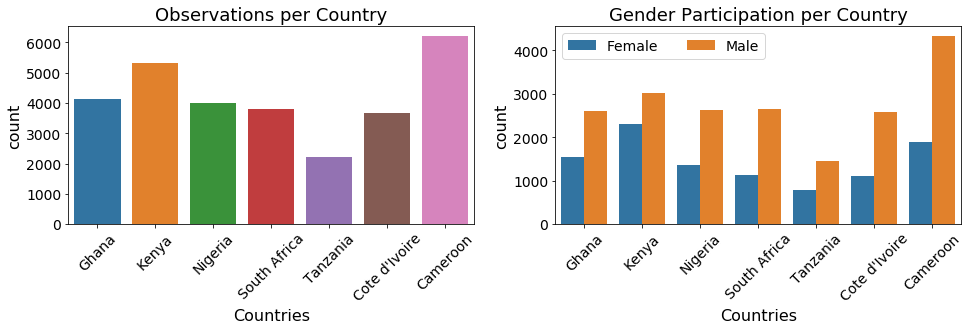
\includegraphics[width=1.15\linewidth]{../../artifacts/obs_per_country} 

}

\caption[Participation per Country]{Participation per Country}\label{fig:pc}
\end{figure}
\end{Schunk}

\begin{Schunk}
\begin{figure}[H]

{\centering 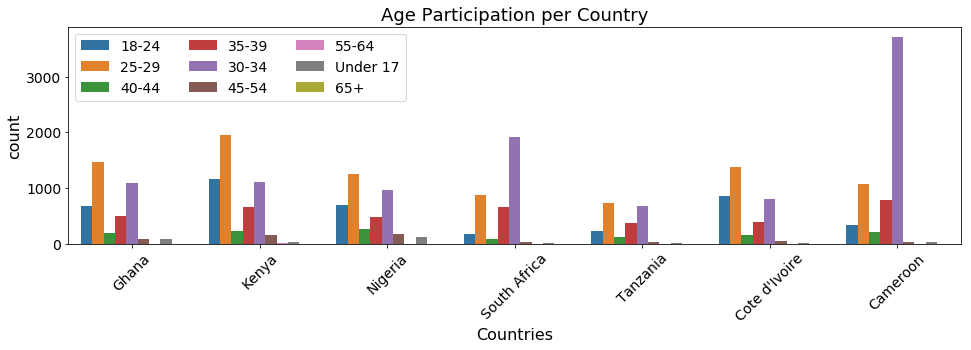
\includegraphics[width=1.15\linewidth]{../../artifacts/participant_age} 

}

\caption[Age of Participans]{Age of Participans}\label{fig:pa}
\end{figure}
\end{Schunk}

\begin{Schunk}
\begin{figure}[H]

{\centering 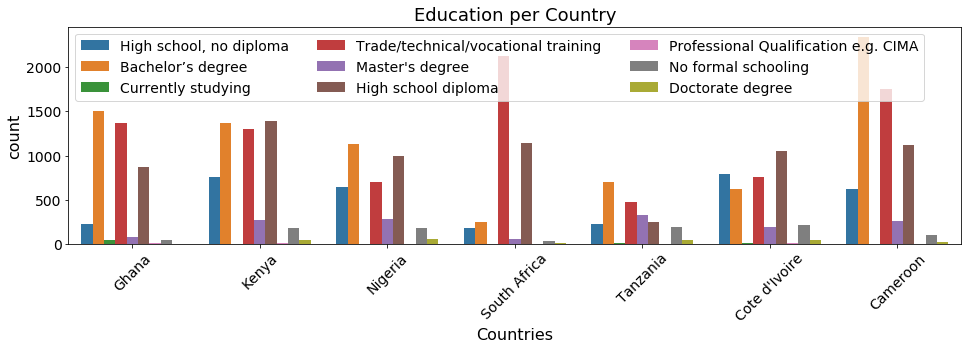
\includegraphics[width=1.15\linewidth]{../../artifacts/participant_education} 

}

\caption[Education of Participants]{Education of Participants}\label{fig:pe}
\end{figure}
\end{Schunk}

\begin{Schunk}
\begin{figure}[H]

{\centering 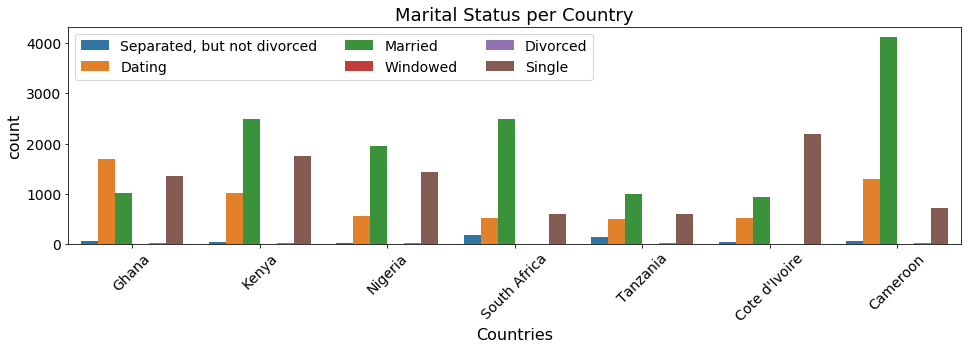
\includegraphics[width=1.15\linewidth]{../../artifacts/participant_marital} 

}

\caption[Marital Status of Participants]{Marital Status of Participants}\label{fig:pms}
\end{figure}
\end{Schunk}

As per the charts submitted above we may conclude that:

\begin{itemize}
\tightlist
\item
  Cameroon has the highest number of observations and Tanzania has the
  smallest representation, while the rest of the countries or more or
  less equally represented.
\item
  Males dominate in the money lending business. Kenya though makes an
  exception where number of female participants is very close to the
  male population
\item
  In general people in \emph{30-34} age group are the most active,
  followed by \emph{25-29} and \emph{18-24} age groups respectively. In
  Kenya, unlike other countries, the younger generation is more active.
\item
  Majority of money lenders are either salaried or commission-based
  employees. Again Kenya makes an exception. The second largest group of
  the money lenders is the business owners.
\item
  Education-wise people with the bachelor's degree and skilled trade
  workers dominate.
\item
  Married people tend to lend money more often\ldots{}
\end{itemize}

\hypertarget{economic-sentiment}{%
\subsubsection{Economic Sentiment}\label{economic-sentiment}}

Now let's see what the money lenders think about the state of the
economy in their respective countries. The questions where asked in the
six-month perspective in the future from the date of survey.

\begin{Schunk}
\begin{figure}[H]

{\centering 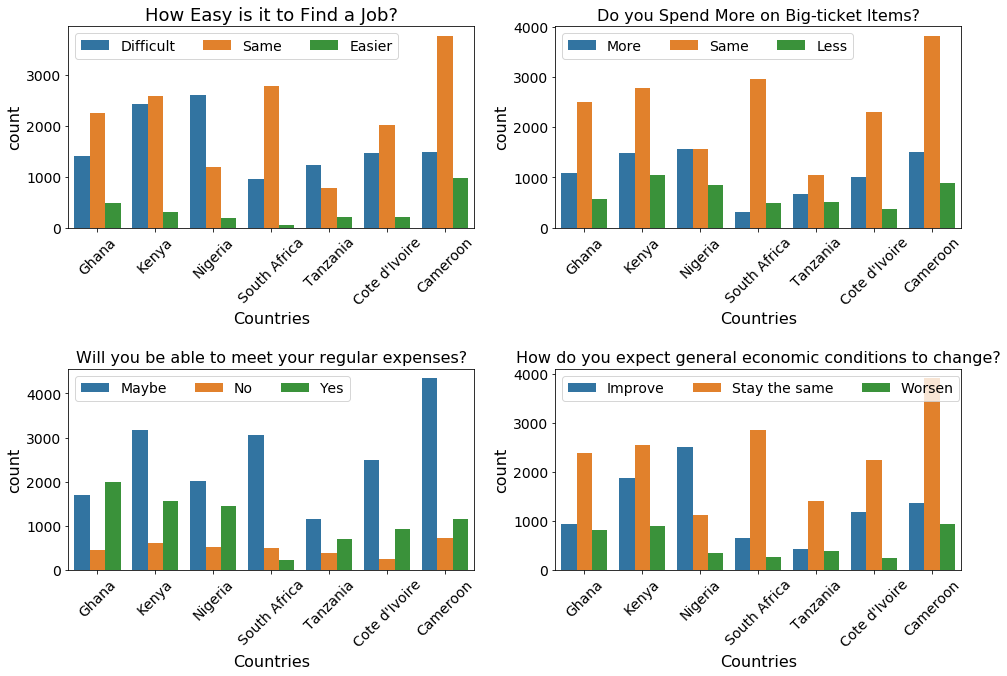
\includegraphics[width=1.15\linewidth]{../../artifacts/sentiment} 

}

\caption[Economic Sentiment]{Economic Sentiment}\label{fig:esent}
\end{figure}
\end{Schunk}

Evidently majority of the survey participants think that the economic
situation in their country will be stable over a course of next six
months. Many people in Kenya, Nigeria and Ghana find it more difficult
to find a job. Remarkably, despite the fact that people believe that the
economic conditions are stable, citizens of all counties are not sure if
they are going to meet their regular expenses.

\hypertarget{spending-and-borrowing-habits}{%
\subsubsection{Spending and Borrowing
Habits}\label{spending-and-borrowing-habits}}

Spending and borrowing habits is the segment of our particular interest
since it affects the most the credit score of the population.

\begin{Schunk}
\begin{figure}[H]

{\centering 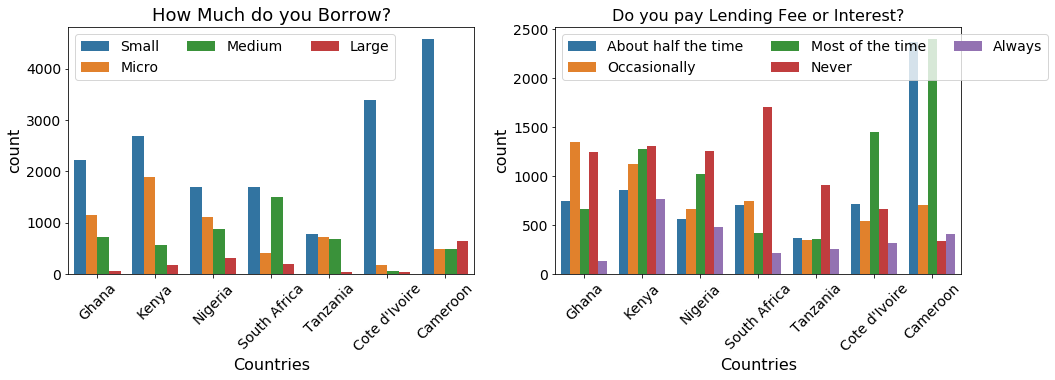
\includegraphics[width=1.15\linewidth]{../../artifacts/borrowing} 

}

\caption[Borrowing Habits]{Borrowing Habits}\label{fig:bh}
\end{figure}
\end{Schunk}

\begin{Schunk}
\begin{figure}[H]

{\centering 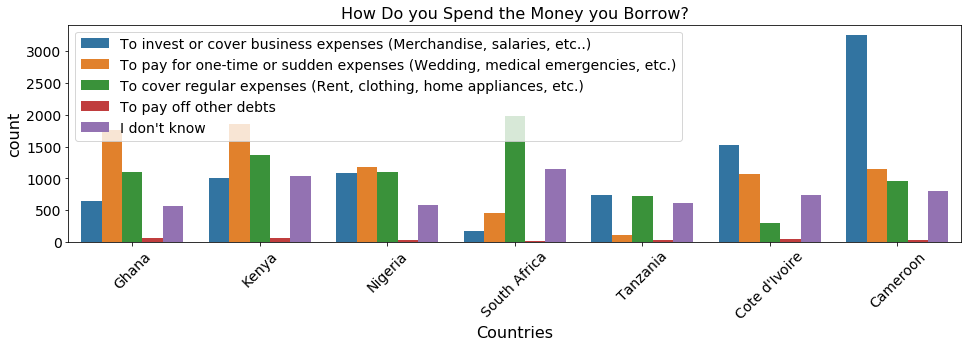
\includegraphics[width=1.15\linewidth]{../../artifacts/spending} 

}

\caption[Spending Habits]{Spending Habits}\label{fig:sh}
\end{figure}
\end{Schunk}

\begin{Schunk}
\begin{figure}[H]

{\centering 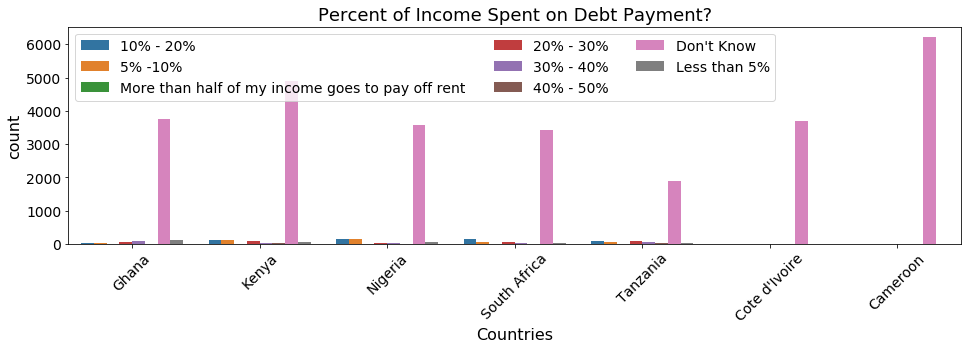
\includegraphics[width=1.15\linewidth]{../../artifacts/payment} 

}

\caption[Debt Payment]{Debt Payment}\label{fig:dtp}
\end{figure}
\end{Schunk}

\begin{itemize}
\tightlist
\item
  Majority of population take either small or micro loans (the exact
  amounts are country specific).
\item
  It is quite remarkable that the lenders do not charge fees or interest
  regularly (if at all) more often than not. The Cameroonians make an
  exception. In opposite the majority of South African lenders never
  charge the interest. We have conducted further data research that have
  proved that many people tend to lend to friends and family. This fact
  explains why the fees and interest on loans are waived.
\item
  People in Cameroon, Cote d'Ivoire and Tanzania spend the loans to
  cover business-related expenses. Citizens of the other countries
  mainly use the loans to either cover one-time/ unexpected expenses
  (wedding, medical emergency..) or make ends meet (pay rent, buy
  clothes, etc.)
\item
  Interestingly people in all countries do not watch how they spend the
  borrowed money. This fact probably explains why the question
  \emph{Will you be able to meet your regular expenses?} generates
  uncertain answers (see \textbf{Economic Sentiment} paragraph for
  further details).
\end{itemize}

\hypertarget{data-distribution-between-categories}{%
\subsection{Data Distribution between
Categories}\label{data-distribution-between-categories}}

There are five credit categories for borrowers and five lender
categories. To train the robust classification models we have to ensure
that each category has enough observations to support the model
training. Let's review the data distribution between the borrower and
lender categories.

\begin{Schunk}
\begin{figure}[H]

{\centering 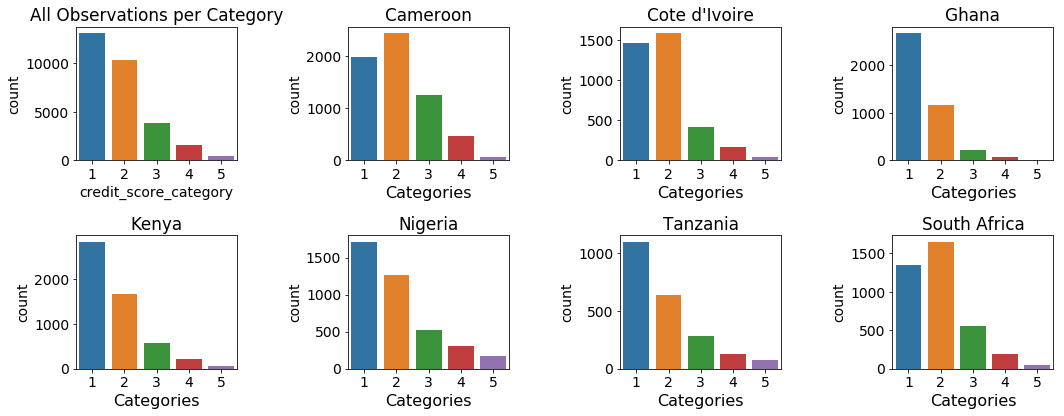
\includegraphics[width=1.15\linewidth]{../../artifacts/bcategories} 

}

\caption[Data Distribution per Credit Categories]{Data Distribution per Credit Categories}\label{fig:dc}
\end{figure}
\end{Schunk}

\begin{Schunk}
\begin{figure}[H]

{\centering 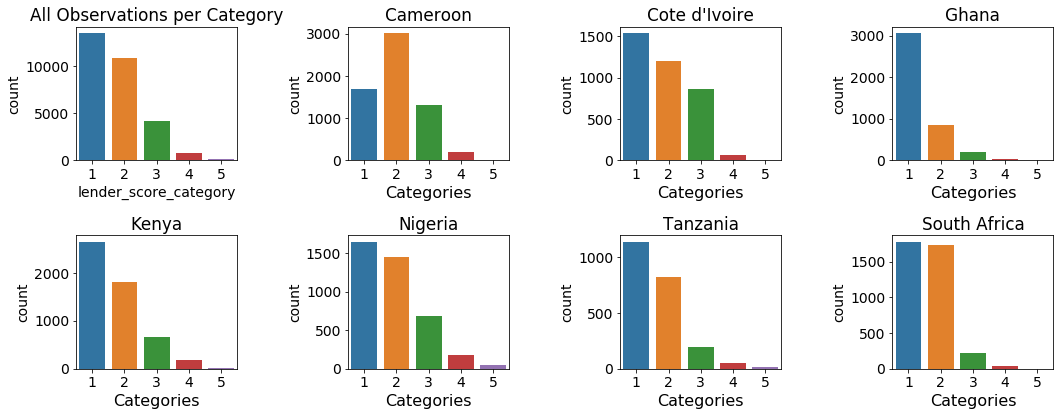
\includegraphics[width=1.15\linewidth]{../../artifacts/lcategories} 

}

\caption[Data Distribution per Lender Categories]{Data Distribution per Lender Categories}\label{fig:dl}
\end{figure}
\end{Schunk}

As we can observe overall the lending environment is not very promising;
categories 1 and 2 (\emph{Very Poor} and \emph{Poor}) dominate. The
lending climate is visibly better in Cameroon, Cote d'Ivoire and South
Africa. It is also worth mentioning that categories 4 and 5 (\emph{Good}
and \emph{Very Good}) do not have that much data. The situation is even
worse with the lender categories. Thus prior to the model training we
would have to upsample the training data sets to bring all categories to
the same level.

Overall looking at the credit and lender scores of the population we
observe that the distribution pattern is very similar between all seven
African countries. Thus if KASI Insight adds more countries to the fold
there is no need to retrain the models assuming that the newly added
countries have the same category distribution\ldots{}

\hypertarget{feature-selection-and-engineering}{%
\section{Feature Selection and
Engineering}\label{feature-selection-and-engineering}}

The data set has 38 columns. We potentially, could employ all of them to
fit the models. But this is not the optimal approach. Not all data
elements contribute to the category identification equally, some may not
contribute at all, so why keep them? Another consideration is that the
large and wide data sets make model training much longer, affect the
accuracy and speed of the models negatively. Also large input variable
set adds complexity to the user interface making it hard to implement,
maintain and use. Thus we have opted to evaluated available data
features. The ultimate goal is to understand the relationship between
the features and the response variables and select the most influential
ones.

\hypertarget{feature-correlation-matrix}{%
\subsection{Feature Correlation
Matrix}\label{feature-correlation-matrix}}

Strongly correlated features are redundant thus they could be dropped
without impacting the model performance. Figure \ref{fig:cmatrix}
depicts a correlation heatmap of all 38 data set features. The
correlated features would be rendered either in deep black or very light
colors. As we can observe none of the features have strong correlation.

\begin{Schunk}
\begin{figure}[H]

{\centering 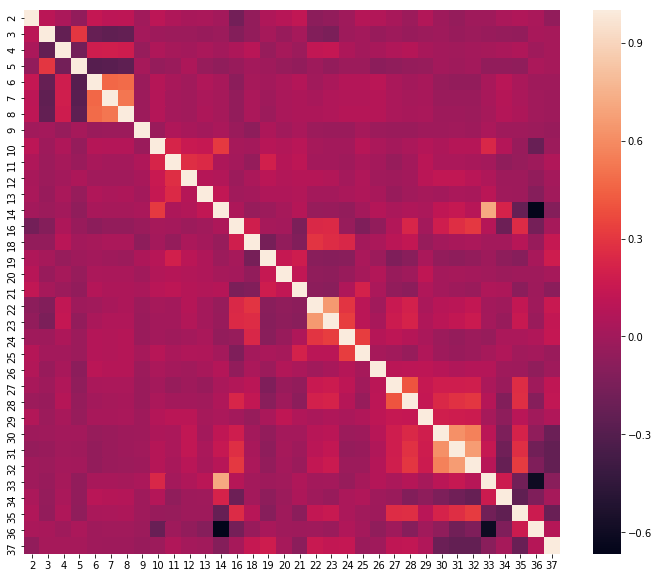
\includegraphics[width=0.75\linewidth]{../../artifacts/cmatrix} 

}

\caption[Feature Correlation]{Feature Correlation}\label{fig:cmatrix}
\end{figure}
\end{Schunk}

\hypertarget{univariate-feature-selection}{%
\subsection{Univariate Feature
Selection}\label{univariate-feature-selection}}

Univariate feature selection examines each feature individually to
determine the strength of the relationship of the feature with the
response variable. Next two paragraphs examine relationship between top
20 features and the credit and lender categories respectively.

\hypertarget{credit-score-univariate-feature-selection}{%
\subsubsection{Credit Score Univariate Feature
Selection}\label{credit-score-univariate-feature-selection}}

\begin{longtable}[]{@{}lll@{}}
\toprule
\begin{minipage}[b]{0.05\columnwidth}\raggedright
Num\strut
\end{minipage} & \begin{minipage}[b]{0.77\columnwidth}\raggedright
Feature\strut
\end{minipage} & \begin{minipage}[b]{0.09\columnwidth}\raggedright
Score\strut
\end{minipage}\tabularnewline
\midrule
\endhead
\begin{minipage}[t]{0.05\columnwidth}\raggedright
24\strut
\end{minipage} & \begin{minipage}[t]{0.77\columnwidth}\raggedright
Do you receive your money back in time?\strut
\end{minipage} & \begin{minipage}[t]{0.09\columnwidth}\raggedright
4749.1\strut
\end{minipage}\tabularnewline
\begin{minipage}[t]{0.05\columnwidth}\raggedright
18\strut
\end{minipage} & \begin{minipage}[t]{0.77\columnwidth}\raggedright
Over the past 3 months, how many times have you lent someone
money?\strut
\end{minipage} & \begin{minipage}[t]{0.09\columnwidth}\raggedright
1077.69\strut
\end{minipage}\tabularnewline
\begin{minipage}[t]{0.05\columnwidth}\raggedright
26\strut
\end{minipage} & \begin{minipage}[t]{0.77\columnwidth}\raggedright
What's the most common use of the money you lend?\strut
\end{minipage} & \begin{minipage}[t]{0.09\columnwidth}\raggedright
727.16\strut
\end{minipage}\tabularnewline
\begin{minipage}[t]{0.05\columnwidth}\raggedright
22\strut
\end{minipage} & \begin{minipage}[t]{0.77\columnwidth}\raggedright
Do you include either interest or a lending fee when you lend?\strut
\end{minipage} & \begin{minipage}[t]{0.09\columnwidth}\raggedright
536.27\strut
\end{minipage}\tabularnewline
\begin{minipage}[t]{0.05\columnwidth}\raggedright
19\strut
\end{minipage} & \begin{minipage}[t]{0.77\columnwidth}\raggedright
On average how much do you lend in general?\strut
\end{minipage} & \begin{minipage}[t]{0.09\columnwidth}\raggedright
512.08\strut
\end{minipage}\tabularnewline
\begin{minipage}[t]{0.05\columnwidth}\raggedright
20\strut
\end{minipage} & \begin{minipage}[t]{0.77\columnwidth}\raggedright
Who did you lend money to in the past 3 months?\strut
\end{minipage} & \begin{minipage}[t]{0.09\columnwidth}\raggedright
441.73\strut
\end{minipage}\tabularnewline
\begin{minipage}[t]{0.05\columnwidth}\raggedright
33\strut
\end{minipage} & \begin{minipage}[t]{0.77\columnwidth}\raggedright
What type of loans are you currently paying of?\strut
\end{minipage} & \begin{minipage}[t]{0.09\columnwidth}\raggedright
360.28\strut
\end{minipage}\tabularnewline
\begin{minipage}[t]{0.05\columnwidth}\raggedright
23\strut
\end{minipage} & \begin{minipage}[t]{0.77\columnwidth}\raggedright
Do you request guarantees when you lend?\strut
\end{minipage} & \begin{minipage}[t]{0.09\columnwidth}\raggedright
351.02\strut
\end{minipage}\tabularnewline
\begin{minipage}[t]{0.05\columnwidth}\raggedright
14\strut
\end{minipage} & \begin{minipage}[t]{0.77\columnwidth}\raggedright
If you are a student, what level are you currently studying?\strut
\end{minipage} & \begin{minipage}[t]{0.09\columnwidth}\raggedright
301.56\strut
\end{minipage}\tabularnewline
\begin{minipage}[t]{0.05\columnwidth}\raggedright
21\strut
\end{minipage} & \begin{minipage}[t]{0.77\columnwidth}\raggedright
When you lend money, when do you usually expect to get it repaid?\strut
\end{minipage} & \begin{minipage}[t]{0.09\columnwidth}\raggedright
218.30\strut
\end{minipage}\tabularnewline
\begin{minipage}[t]{0.05\columnwidth}\raggedright
16\strut
\end{minipage} & \begin{minipage}[t]{0.77\columnwidth}\raggedright
Country\strut
\end{minipage} & \begin{minipage}[t]{0.09\columnwidth}\raggedright
197.034\strut
\end{minipage}\tabularnewline
\begin{minipage}[t]{0.05\columnwidth}\raggedright
25\strut
\end{minipage} & \begin{minipage}[t]{0.77\columnwidth}\raggedright
Assuming that you have lent money at least ten times, how often would
you get your money repaid?\strut
\end{minipage} & \begin{minipage}[t]{0.09\columnwidth}\raggedright
180.84\strut
\end{minipage}\tabularnewline
\begin{minipage}[t]{0.05\columnwidth}\raggedright
11\strut
\end{minipage} & \begin{minipage}[t]{0.77\columnwidth}\raggedright
Age\strut
\end{minipage} & \begin{minipage}[t]{0.09\columnwidth}\raggedright
103.30\strut
\end{minipage}\tabularnewline
\begin{minipage}[t]{0.05\columnwidth}\raggedright
12\strut
\end{minipage} & \begin{minipage}[t]{0.77\columnwidth}\raggedright
What's your highest level of education?\strut
\end{minipage} & \begin{minipage}[t]{0.09\columnwidth}\raggedright
75.24\strut
\end{minipage}\tabularnewline
\begin{minipage}[t]{0.05\columnwidth}\raggedright
29\strut
\end{minipage} & \begin{minipage}[t]{0.77\columnwidth}\raggedright
What is the most convenient way to get a loan?\strut
\end{minipage} & \begin{minipage}[t]{0.09\columnwidth}\raggedright
63.37\strut
\end{minipage}\tabularnewline
\begin{minipage}[t]{0.05\columnwidth}\raggedright
2\strut
\end{minipage} & \begin{minipage}[t]{0.77\columnwidth}\raggedright
Has it become more difficult or easier to find a job in your city?\strut
\end{minipage} & \begin{minipage}[t]{0.09\columnwidth}\raggedright
55.15\strut
\end{minipage}\tabularnewline
\begin{minipage}[t]{0.05\columnwidth}\raggedright
10\strut
\end{minipage} & \begin{minipage}[t]{0.77\columnwidth}\raggedright
Marital status\strut
\end{minipage} & \begin{minipage}[t]{0.09\columnwidth}\raggedright
39.54\strut
\end{minipage}\tabularnewline
\begin{minipage}[t]{0.05\columnwidth}\raggedright
31\strut
\end{minipage} & \begin{minipage}[t]{0.77\columnwidth}\raggedright
To what extent do you agree with the following sentences {[}Credit is
beneficial only if you h\ldots{}\strut
\end{minipage} & \begin{minipage}[t]{0.09\columnwidth}\raggedright
35.68\strut
\end{minipage}\tabularnewline
\begin{minipage}[t]{0.05\columnwidth}\raggedright
30\strut
\end{minipage} & \begin{minipage}[t]{0.77\columnwidth}\raggedright
To what extent do you agree with the following sentences {[}Access to
credit is essential for \ldots{}\strut
\end{minipage} & \begin{minipage}[t]{0.09\columnwidth}\raggedright
31.48\strut
\end{minipage}\tabularnewline
\begin{minipage}[t]{0.05\columnwidth}\raggedright
32\strut
\end{minipage} & \begin{minipage}[t]{0.77\columnwidth}\raggedright
To what extent do you agree with the following sentences {[}I would like
to have more credit m\ldots{}\strut
\end{minipage} & \begin{minipage}[t]{0.09\columnwidth}\raggedright
25.52\strut
\end{minipage}\tabularnewline
\bottomrule
\end{longtable}

\hypertarget{lender-score-univariate-feature-selection}{%
\subsubsection{Lender Score Univariate Feature
Selection}\label{lender-score-univariate-feature-selection}}

\begin{longtable}[]{@{}lll@{}}
\toprule
\begin{minipage}[b]{0.05\columnwidth}\raggedright
Num\strut
\end{minipage} & \begin{minipage}[b]{0.77\columnwidth}\raggedright
Feature\strut
\end{minipage} & \begin{minipage}[b]{0.09\columnwidth}\raggedright
Score\strut
\end{minipage}\tabularnewline
\midrule
\endhead
\begin{minipage}[t]{0.05\columnwidth}\raggedright
24\strut
\end{minipage} & \begin{minipage}[t]{0.77\columnwidth}\raggedright
Do you receive your money back in time?\strut
\end{minipage} & \begin{minipage}[t]{0.09\columnwidth}\raggedright
6667.83\strut
\end{minipage}\tabularnewline
\begin{minipage}[t]{0.05\columnwidth}\raggedright
22\strut
\end{minipage} & \begin{minipage}[t]{0.77\columnwidth}\raggedright
Do you include either interest or a lending fee when you lend?\strut
\end{minipage} & \begin{minipage}[t]{0.09\columnwidth}\raggedright
3588.47\strut
\end{minipage}\tabularnewline
\begin{minipage}[t]{0.05\columnwidth}\raggedright
23\strut
\end{minipage} & \begin{minipage}[t]{0.77\columnwidth}\raggedright
Do you request guarantees when you lend?\strut
\end{minipage} & \begin{minipage}[t]{0.09\columnwidth}\raggedright
3339.37\strut
\end{minipage}\tabularnewline
\begin{minipage}[t]{0.05\columnwidth}\raggedright
18\strut
\end{minipage} & \begin{minipage}[t]{0.77\columnwidth}\raggedright
Over the past 3 months, how many times have you lent someone
money?\strut
\end{minipage} & \begin{minipage}[t]{0.09\columnwidth}\raggedright
2014.33\strut
\end{minipage}\tabularnewline
\begin{minipage}[t]{0.05\columnwidth}\raggedright
16\strut
\end{minipage} & \begin{minipage}[t]{0.77\columnwidth}\raggedright
Country\strut
\end{minipage} & \begin{minipage}[t]{0.09\columnwidth}\raggedright
595.87\strut
\end{minipage}\tabularnewline
\begin{minipage}[t]{0.05\columnwidth}\raggedright
25\strut
\end{minipage} & \begin{minipage}[t]{0.77\columnwidth}\raggedright
Assuming that you have lent money at least ten times, how often would
you get your money repaid?\strut
\end{minipage} & \begin{minipage}[t]{0.09\columnwidth}\raggedright
555.59\strut
\end{minipage}\tabularnewline
\begin{minipage}[t]{0.05\columnwidth}\raggedright
19\strut
\end{minipage} & \begin{minipage}[t]{0.77\columnwidth}\raggedright
On average how much do you lend in general?\strut
\end{minipage} & \begin{minipage}[t]{0.09\columnwidth}\raggedright
460.15\strut
\end{minipage}\tabularnewline
\begin{minipage}[t]{0.05\columnwidth}\raggedright
26\strut
\end{minipage} & \begin{minipage}[t]{0.77\columnwidth}\raggedright
What's the most common use of the money you lend?\strut
\end{minipage} & \begin{minipage}[t]{0.09\columnwidth}\raggedright
444.85\strut
\end{minipage}\tabularnewline
\begin{minipage}[t]{0.05\columnwidth}\raggedright
20\strut
\end{minipage} & \begin{minipage}[t]{0.77\columnwidth}\raggedright
Who did you lend money to in the past 3 months?\strut
\end{minipage} & \begin{minipage}[t]{0.09\columnwidth}\raggedright
415.17\strut
\end{minipage}\tabularnewline
\begin{minipage}[t]{0.05\columnwidth}\raggedright
14\strut
\end{minipage} & \begin{minipage}[t]{0.77\columnwidth}\raggedright
If you are a student, what level are you currently studying?\strut
\end{minipage} & \begin{minipage}[t]{0.09\columnwidth}\raggedright
174.17\strut
\end{minipage}\tabularnewline
\begin{minipage}[t]{0.05\columnwidth}\raggedright
21\strut
\end{minipage} & \begin{minipage}[t]{0.77\columnwidth}\raggedright
When you lend money, when do you usually expect to get it repaid?\strut
\end{minipage} & \begin{minipage}[t]{0.09\columnwidth}\raggedright
112.94\strut
\end{minipage}\tabularnewline
\begin{minipage}[t]{0.05\columnwidth}\raggedright
37\strut
\end{minipage} & \begin{minipage}[t]{0.77\columnwidth}\raggedright
If you wanted to take a loan to start a business, how much would you
need?\strut
\end{minipage} & \begin{minipage}[t]{0.09\columnwidth}\raggedright
91.9\strut
\end{minipage}\tabularnewline
\begin{minipage}[t]{0.05\columnwidth}\raggedright
28\strut
\end{minipage} & \begin{minipage}[t]{0.77\columnwidth}\raggedright
Are you a tontine / lending club member?\strut
\end{minipage} & \begin{minipage}[t]{0.09\columnwidth}\raggedright
78.77\strut
\end{minipage}\tabularnewline
\begin{minipage}[t]{0.05\columnwidth}\raggedright
27\strut
\end{minipage} & \begin{minipage}[t]{0.77\columnwidth}\raggedright
Have you ever applied for a bank loan?\strut
\end{minipage} & \begin{minipage}[t]{0.09\columnwidth}\raggedright
76.69\strut
\end{minipage}\tabularnewline
\begin{minipage}[t]{0.05\columnwidth}\raggedright
4\strut
\end{minipage} & \begin{minipage}[t]{0.77\columnwidth}\raggedright
Compared to the last 6 months, are you able to spend (more, the same or
less) money on large pur\ldots{}\strut
\end{minipage} & \begin{minipage}[t]{0.09\columnwidth}\raggedright
56.49\strut
\end{minipage}\tabularnewline
\begin{minipage}[t]{0.05\columnwidth}\raggedright
11\strut
\end{minipage} & \begin{minipage}[t]{0.77\columnwidth}\raggedright
Age\strut
\end{minipage} & \begin{minipage}[t]{0.09\columnwidth}\raggedright
44.33\strut
\end{minipage}\tabularnewline
\begin{minipage}[t]{0.05\columnwidth}\raggedright
8\strut
\end{minipage} & \begin{minipage}[t]{0.77\columnwidth}\raggedright
How do you expect general economic conditions in your country to change
over the next 6 months?\strut
\end{minipage} & \begin{minipage}[t]{0.09\columnwidth}\raggedright
42.94\strut
\end{minipage}\tabularnewline
\begin{minipage}[t]{0.05\columnwidth}\raggedright
32\strut
\end{minipage} & \begin{minipage}[t]{0.77\columnwidth}\raggedright
To what extent do you agree with the following sentences {[}I would like
to have more credit manag\ldots{}\strut
\end{minipage} & \begin{minipage}[t]{0.09\columnwidth}\raggedright
39.22\strut
\end{minipage}\tabularnewline
\begin{minipage}[t]{0.05\columnwidth}\raggedright
2\strut
\end{minipage} & \begin{minipage}[t]{0.77\columnwidth}\raggedright
Has it become more difficult or easier to find a job in your city?\strut
\end{minipage} & \begin{minipage}[t]{0.09\columnwidth}\raggedright
38.57\strut
\end{minipage}\tabularnewline
\begin{minipage}[t]{0.05\columnwidth}\raggedright
35\strut
\end{minipage} & \begin{minipage}[t]{0.77\columnwidth}\raggedright
Do you have a credit card?\strut
\end{minipage} & \begin{minipage}[t]{0.09\columnwidth}\raggedright
37.26\strut
\end{minipage}\tabularnewline
\bottomrule
\end{longtable}

\hypertarget{feature-importance}{%
\subsection{Feature Importance}\label{feature-importance}}

We measure the importance of a feature by calculating the increase in
the model's prediction error after permuting the feature. A feature is
``important'' if shuffling its values increases the model error, because
in this case the model relied on the feature for the prediction. A
feature is ``unimportant'' if shuffling its values leaves the model
error unchanged, because in this case the model ignored the feature for
the prediction.

\hypertarget{credit-score-feature-importance-evaluation}{%
\subsubsection{Credit Score Feature Importance
Evaluation}\label{credit-score-feature-importance-evaluation}}

\begin{Schunk}
\begin{figure}[H]

{\centering 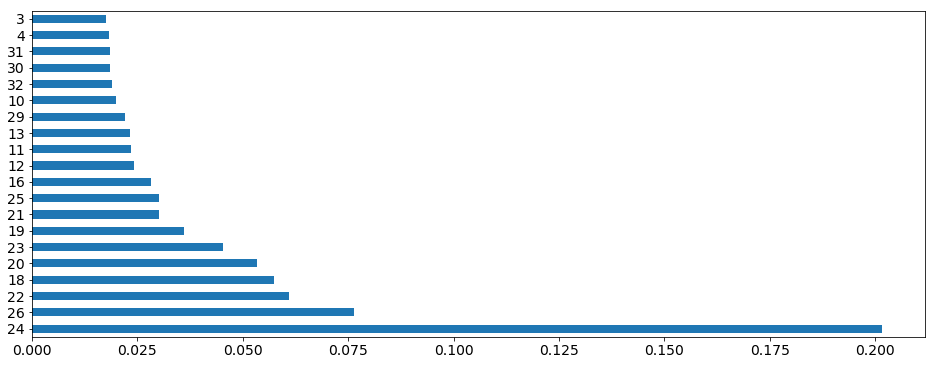
\includegraphics[width=1\linewidth]{../../artifacts/cfimportance} 

}

\caption[Credit Score Feature Impoirtance]{Credit Score Feature Impoirtance}\label{fig:cfi}
\end{figure}
\end{Schunk}

\hypertarget{lender-score-feature-importance-evaluation}{%
\subsubsection{Lender Score Feature Importance
Evaluation}\label{lender-score-feature-importance-evaluation}}

\begin{Schunk}
\begin{figure}[H]

{\centering 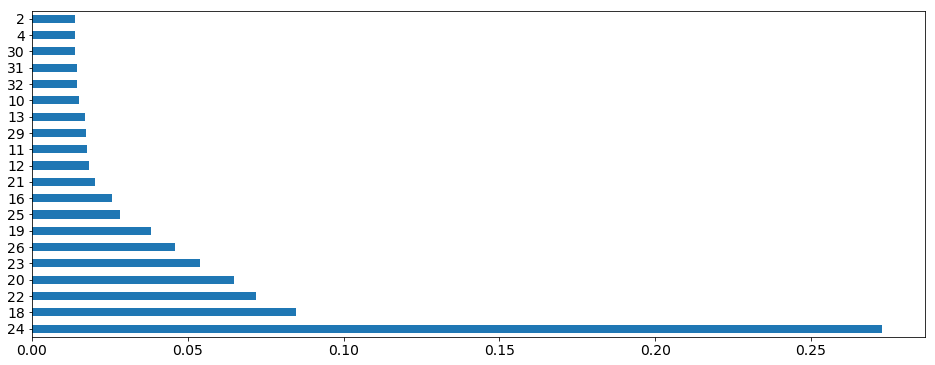
\includegraphics[width=1\linewidth]{../../artifacts/lfimportance} 

}

\caption[Lender Score Feature Impoirtance]{Lender Score Feature Impoirtance}\label{fig:lfi}
\end{figure}
\end{Schunk}

\hypertarget{takeaways}{%
\subsection{Takeaways}\label{takeaways}}

We have applied two mathematical algorithms to identify the most
significant features for credit score and lender score labels. To no
surprise both methods have successfully identified the feature that have
been used to calculate the credit/ lender categories. We have selected
the top features that have distinctively higher score as the base-line
features sets. During the model training and evaluation phase we will
increase/decrease the number of features to estimate the effect of the
input data dimentionality change on the model accuracy.

\hypertarget{top-seven-credit-score-features}{%
\subsubsection{Top Seven Credit Score
Features}\label{top-seven-credit-score-features}}

\begin{longtable}[]{@{}ll@{}}
\toprule
Num & Feature\tabularnewline
\midrule
\endhead
24 & Do you receive your money back in time?\tabularnewline
26 & What's the most common use of the money you lend?\tabularnewline
22 & Do you include either interest or a lending fee when you
lend?\tabularnewline
18 & Over the past 3 months, how many times have you lent someone
money?\tabularnewline
20 & Who did you lend money to in the past 3 months?\tabularnewline
23 & Do you request guarantees when you lend?\tabularnewline
19 & On average how much do you lend in general?\tabularnewline
\bottomrule
\end{longtable}

\hypertarget{top-nine-lender-score-features}{%
\subsubsection{Top Nine Lender Score
Features}\label{top-nine-lender-score-features}}

\begin{longtable}[]{@{}ll@{}}
\toprule
\begin{minipage}[b]{0.05\columnwidth}\raggedright
Num\strut
\end{minipage} & \begin{minipage}[b]{0.89\columnwidth}\raggedright
Feature\strut
\end{minipage}\tabularnewline
\midrule
\endhead
\begin{minipage}[t]{0.05\columnwidth}\raggedright
24\strut
\end{minipage} & \begin{minipage}[t]{0.89\columnwidth}\raggedright
Do you receive your money back in time?\strut
\end{minipage}\tabularnewline
\begin{minipage}[t]{0.05\columnwidth}\raggedright
18\strut
\end{minipage} & \begin{minipage}[t]{0.89\columnwidth}\raggedright
Over the past 3 months, how many times have you lent someone
money?\strut
\end{minipage}\tabularnewline
\begin{minipage}[t]{0.05\columnwidth}\raggedright
22\strut
\end{minipage} & \begin{minipage}[t]{0.89\columnwidth}\raggedright
Do you include either interest or a lending fee when you lend?\strut
\end{minipage}\tabularnewline
\begin{minipage}[t]{0.05\columnwidth}\raggedright
23\strut
\end{minipage} & \begin{minipage}[t]{0.89\columnwidth}\raggedright
Do you request guarantees when you lend?\strut
\end{minipage}\tabularnewline
\begin{minipage}[t]{0.05\columnwidth}\raggedright
20\strut
\end{minipage} & \begin{minipage}[t]{0.89\columnwidth}\raggedright
Who did you lend money to in the past 3 months?\strut
\end{minipage}\tabularnewline
\begin{minipage}[t]{0.05\columnwidth}\raggedright
26\strut
\end{minipage} & \begin{minipage}[t]{0.89\columnwidth}\raggedright
What's the most common use of the money you lend?\strut
\end{minipage}\tabularnewline
\begin{minipage}[t]{0.05\columnwidth}\raggedright
19\strut
\end{minipage} & \begin{minipage}[t]{0.89\columnwidth}\raggedright
On average how much do you lend in general?\strut
\end{minipage}\tabularnewline
\begin{minipage}[t]{0.05\columnwidth}\raggedright
25\strut
\end{minipage} & \begin{minipage}[t]{0.89\columnwidth}\raggedright
Assuming that you have lent money at least ten times, how often would
you get your money repaid?\strut
\end{minipage}\tabularnewline
\begin{minipage}[t]{0.05\columnwidth}\raggedright
16\strut
\end{minipage} & \begin{minipage}[t]{0.89\columnwidth}\raggedright
Country\strut
\end{minipage}\tabularnewline
\bottomrule
\end{longtable}

\hypertarget{model-evaluation-and-selection}{%
\subsection{Model Evaluation and
Selection}\label{model-evaluation-and-selection}}

After we cleaned and normalized the data, labeled all observations and
gained deep understanding about the features we are ready to start model
training and evaluation. To achieve the best result possible we will
explore and evaluate three algorithms to train the models. They are:

\begin{itemize}
\tightlist
\item
  \textbf{Support Vector Machine} (SVM). The greatest strength of SVM is
  that it has multiple Kernel implementations, that could be tuned to
  explain multi-dimensional space with high accuracy.
\item
  \textbf{Random Forest} (RF). Random forest belongs to the class of
  ensemble models. It has many hyper-parameters that could be tuned to
  achieve high accuracy. The random forest algorithm is not demanding in
  terms of the data preparation, which makes it the first choice in many
  real-life scenarios.
\item
  \textbf{Gradient Boosting Machine} (GBM). GBM is an ensemble model as
  well. It uses the concept of trees just like the RF model does but
  applies it differently. GBM builds the trees one at a time, where each
  new tree helps to correct errors made by previously trained tree.
\end{itemize}

\hypertarget{evaluation-metrics}{%
\subsubsection{Evaluation Metrics}\label{evaluation-metrics}}

We believe that the best model has to classify all five categories as
accurate as possible. The winning model also would have to identify true
positives and true negatives for each category equally well. Thus we
choose the multiclass confusion matrix and F1 scores to evaluate the
models. The higher the F1 score for each category - the better the model
performs. We also take into consideration the model training and
inference speed.

\hypertarget{model-training-and-evaluation-methodology}{%
\subsubsection{Model Training and Evaluation
Methodology}\label{model-training-and-evaluation-methodology}}

\begin{itemize}
\tightlist
\item
  For the base-line model training we will use top seven feature for the
  simulator and top nine feature for the evaluator.
\item
  We begin with the splitting the available data into the training
  (70\%) and test (30\%) sets. We make sure that the training set has
  all categories represented proportionally to the original data set.
\item
  We upsample the training data set employing \emph{SMOTE} algorithm
  (Ref:\cite{smote}).
\item
  We evaluate the three algorithms we have described above. We will be
  using the default algorithm parameters and top features (see
  \emph{Feature Evaluation} paragraph for more details) to fit the
  models.
\item
  We select the algorithm that has the best evaluation metrics.
\item
  Then we evaluate the winning algorithm fitting it with the smaller and
  larger feature sets.
\item
  If the data dimentionality change makes positive impact on the the
  winning algorithm we select this feature set for the model.
\item
  Finally we hyper-tune the algorithm parameters in effort to achieve
  even better model performance
\end{itemize}

\hypertarget{upsampled-training-data-sets}{%
\subsubsection{Upsampled Training Data
Sets}\label{upsampled-training-data-sets}}

Let's take a quick look at the training sets after we applied
\texttt{SMOTE} upsampling algorithm.

\begin{longtable}[]{@{}ll@{}}
\toprule
Simulator Model Training Set Size & Evaluator Model Training Set
Size\tabularnewline
\midrule
\endhead
\textbf{45895} & \textbf{47330}\tabularnewline
\bottomrule
\end{longtable}

\begin{Schunk}
\begin{figure}[H]

{\centering 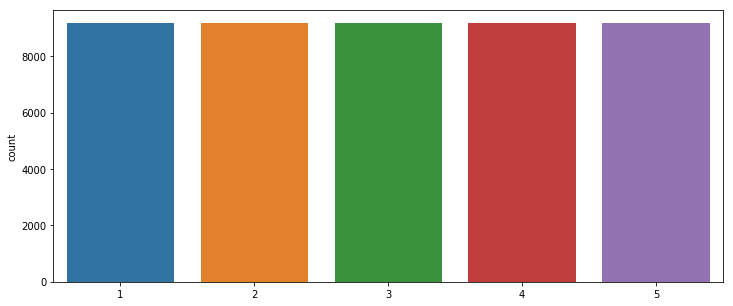
\includegraphics[width=0.49\linewidth,height=0.2\textheight]{../../artifacts/upsampled_simulator} 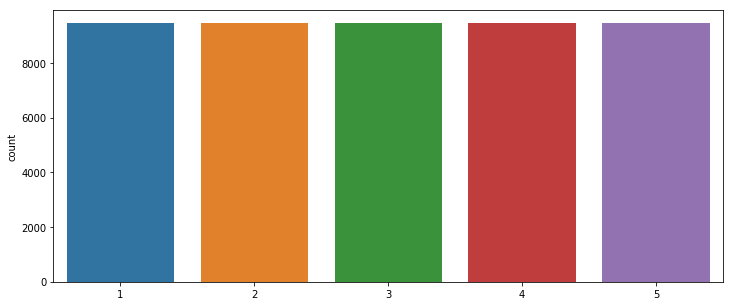
\includegraphics[width=0.49\linewidth,height=0.2\textheight]{../../artifacts/upsampled_evaluator} 

}

\caption[Upsampled Training Data Sets per Category for Sampler and Evaluator]{Upsampled Training Data Sets per Category for Sampler and Evaluator}\label{fig:upsampled}
\end{figure}
\end{Schunk}

\hypertarget{lending-environment-simulator-model}{%
\subsubsection{Lending Environment Simulator
Model}\label{lending-environment-simulator-model}}

Following the steps outlined in the previous section we have received
the following performances stats:

\hypertarget{svm}{%
\paragraph{SVM}\label{svm}}

\begin{verbatim}
              precision    recall  f1-score   support
       1       0.97      0.95      0.96      3935
       2       0.92      0.90      0.91      3114
       3       0.81      0.89      0.85      1122
       4       0.81      0.85      0.83       487
       5       0.81      0.89      0.85       157
       
micro avg      0.92      0.92      0.92      8815
macro avg      0.86      0.90      0.88      8815
weighted avg   0.92      0.92      0.92      8815

Overall algorithm accuracy: 0.9199
\end{verbatim}

\hypertarget{random-forest}{%
\paragraph{Random Forest}\label{random-forest}}

\begin{verbatim}
              precision    recall  f1-score   support
       1       0.98      0.96      0.97      3902
       2       0.93      0.93      0.93      3161
       3       0.86      0.90      0.88      1150
       4       0.86      0.84      0.85       464
       5       0.86      0.87      0.87       138
       
 micro avg     0.94      0.94      0.94      8815
 macro avg     0.90      0.90      0.90      8815
 weighted avg  0.94      0.94      0.94      8815
 
 Overall algorithm accuracy: 0.9372
\end{verbatim}

\hypertarget{gradient-boosting}{%
\paragraph{Gradient Boosting}\label{gradient-boosting}}

\begin{verbatim}
          precision    recall  f1-score   support
       1       0.98      0.92      0.95      3948
       2       0.85      0.87      0.86      3117
       3       0.70      0.67      0.69      1149
       4       0.60      0.82      0.70       471
       5       0.60      0.88      0.71       130
       
 micro avg     0.86      0.86      0.86      8815
 macro avg     0.75      0.83      0.78      8815
 weighted avg  0.87      0.86      0.87      8815
 
 Overall algorithm accuracy: 0.8635
\end{verbatim}

\hypertarget{the-best-lending-environment-simulator-model}{%
\subsubsection{The Best Lending Environment Simulator
Model}\label{the-best-lending-environment-simulator-model}}

The \textbf{Random Forest} algorithm has come up on top. This model
classifies all categories much better than the other two algorithms and
demonstrates a nice balance between the recall and precision metrics.
The Random forest algorithm is also the fastest to train.

\begin{longtable}[]{@{}llll@{}}
\toprule
Category & \textbf{RF f1-score} & SVM f1-score & GB
f1-score\tabularnewline
\midrule
\endhead
1 & \textbf{0.97} & 0.96 & 0.95\tabularnewline
2 & \textbf{0.93} & 0.91 & 0.86\tabularnewline
3 & \textbf{0.88} & 0.85 & 0.69\tabularnewline
4 & \textbf{0.85} & 0.83 & 0.70\tabularnewline
5 & \textbf{0.87} & 0.85 & 0.71\tabularnewline
Accuracy & \textbf{0.9372} & 0.9199 & 0.8635\tabularnewline
\bottomrule
\end{longtable}

\hypertarget{dimensionality-change}{%
\subsubsection{Dimensionality Change}\label{dimensionality-change}}

The winning algorithm performs quite spectacular. It employs the
\textbf{seven} top features we have identified in the \emph{Feature
Selection} section. Let's see how the input data dimentionality change
affects the model performance. Firstly we reduce the number of features
to \textbf{five}.

Top five features

\begin{longtable}[]{@{}ll@{}}
\toprule
Num & Feature\tabularnewline
\midrule
\endhead
24 & Do you receive your money back in time?\tabularnewline
26 & What's the most common use of the money you lend?\tabularnewline
22 & Do you include either interest or a lending fee when you
lend?\tabularnewline
18 & Over the past 3 months, how many times have you lent someone
money?\tabularnewline
20 & Who did you lend money to in the past 3 months?\tabularnewline
\bottomrule
\end{longtable}

Model Performance:

\begin{verbatim}
         precision    recall  f1-score   support
       1       0.94      0.91      0.92      3858
       2       0.84      0.74      0.79      3150
       3       0.58      0.73      0.65      1210
       4       0.55      0.71      0.62       464
       5       0.55      0.89      0.68       133

micro avg      0.81      0.81      0.81      8815
macro avg      0.69      0.80      0.73      8815
weighted avg   0.83      0.81      0.82      8815

Overall algorithm accuracy: 0.8635
\end{verbatim}

Evidently the dimentionality reduction caused the model performance
deteriorate greatly. Now let's increase the number of features to
\textbf{nine}.

Top nine features:

\begin{longtable}[]{@{}ll@{}}
\toprule
Num & Feature\tabularnewline
\midrule
\endhead
24 & Do you receive your money back in time?\tabularnewline
26 & What's the most common use of the money you lend?\tabularnewline
22 & Do you include either interest or a lending fee when you
lend?\tabularnewline
18 & Over the past 3 months, how many times have you lent someone
money?\tabularnewline
20 & Who did you lend money to in the past 3 months?\tabularnewline
23 & Do you request guarantees when you lend?\tabularnewline
19 & On average how much do you lend in general?\tabularnewline
16 & Country\tabularnewline
21 & When you lend money, when do you usually expect to get it
repaid?\tabularnewline
\bottomrule
\end{longtable}

Model Performance:

\begin{verbatim}
          precision    recall  f1-score   support

       1       0.99      0.98      0.98      3893
       2       0.96      0.96      0.96      3159
       3       0.89      0.92      0.91      1151
       4       0.85      0.87      0.86       482
       5       0.88      0.88      0.88       130

 micro avg     0.95      0.95      0.95      8815
 macro avg     0.91      0.92      0.92      8815
 weighted avg  0.96      0.95      0.95      8815
 
 Overall algorithm accuracy: 0.9547
\end{verbatim}

The dimentionality increase gave us a performance boost of almost
\textbf{2\%}. It might not seem much. Let see how the identification of
each category by the model has been affected.

\begin{longtable}[]{@{}lllll@{}}
\toprule
Category & 5 Features & 7 Features (base line) & \textbf{9 Features} &
Gain (\%)\tabularnewline
\midrule
\endhead
1 & 0.92 & 0.96 & \textbf{0.98} & 2\tabularnewline
2 & 0.79 & 0.93 & \textbf{0.96} & 3\tabularnewline
3 & 0.65 & 0.88 & \textbf{0.91} & 3\tabularnewline
4 & 0.62 & 0.85 & \textbf{0.86} & 1\tabularnewline
5 & 0.68 & 0.87 & \textbf{0.88} & 1\tabularnewline
\bottomrule
\end{longtable}

Evidently categories 2 (\emph{Poor}) and 3 (\emph{Fair}) have benefited
the most form the dimentionality increase. Ultimately it is up to the
business to decide if 2\% accuracy gain is worth the training time and
user interface complexity increase. KASI Insight team has opted for the
higher accuracy.

\hypertarget{hyper-parameter-tuning}{%
\subsubsection{Hyper-parameter Tuning}\label{hyper-parameter-tuning}}

The hyper-parameter tuning is usually the last step in effort to improve
the model performance. We will employ \emph{Grid Search} algorithm with
\textbf{three-fold cross validation} to identify the best model
parameters. The parameter grid look as follows:

\begin{longtable}[]{@{}ll@{}}
\toprule
Parameter & Values\tabularnewline
\midrule
\endhead
Number of Estimators & 200, 300, 400\tabularnewline
Minimum Sample Split & 5, 10, 20, 30, 40\tabularnewline
Maximum Features & `auto', `sqrt'\tabularnewline
Bootstrap: & True, False\tabularnewline
\bottomrule
\end{longtable}

The hyper-parameter tuning gave us another \textbf{0.5\%} performance
gain.

\hypertarget{final-simulator-model-stats}{%
\subsubsection{Final Simulator Model
Stats}\label{final-simulator-model-stats}}

\begin{itemize}
\tightlist
\item
  Number of features: \textbf{9}
\item
  Overall algorithm accuracy: \textbf{0.9594}
\end{itemize}

\begin{Schunk}
\begin{figure}[H]

{\centering 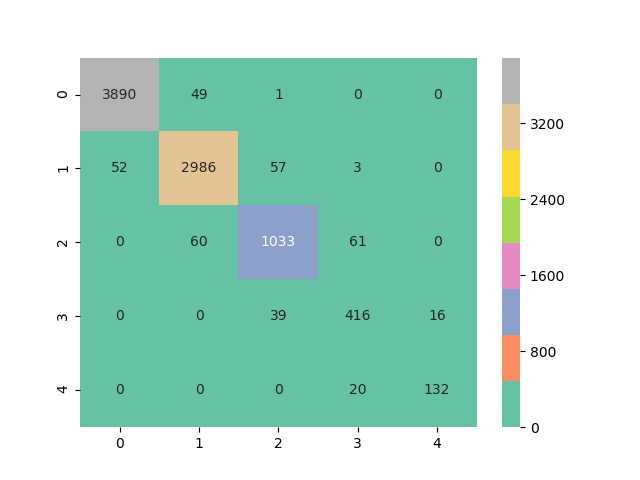
\includegraphics[width=0.9\linewidth]{../../models/training/simulator_rf_tuned_large_matrix} 

}

\caption[Simulator Model Confusion Matrix]{Simulator Model Confusion Matrix}\label{fig:simulator_cm}
\end{figure}
\end{Schunk}

\begin{verbatim}
          precision    recall  f1-score   support

       1       0.99      0.99      0.99      3940
       2       0.96      0.96      0.96      3098
       3       0.91      0.90      0.90      1154
       4       0.83      0.88      0.86       471
       5       0.89      0.87      0.88       152

 micro avg     0.96      0.96      0.96      8815
 macro avg     0.92      0.92      0.92      8815
 weighted avg  0.96      0.96      0.96      8815
\end{verbatim}

Lastly we are going to review the model learning and validation curves.
As per figure \ref{fig:simulator_lc} the model was learning more about
the data as the training size grew. When the training size reached about
30,000 observations the validation curve converged with the training one
indicating that the further increase in the training set size will not
likely result in better model performance.

\begin{Schunk}
\begin{figure}[H]

{\centering 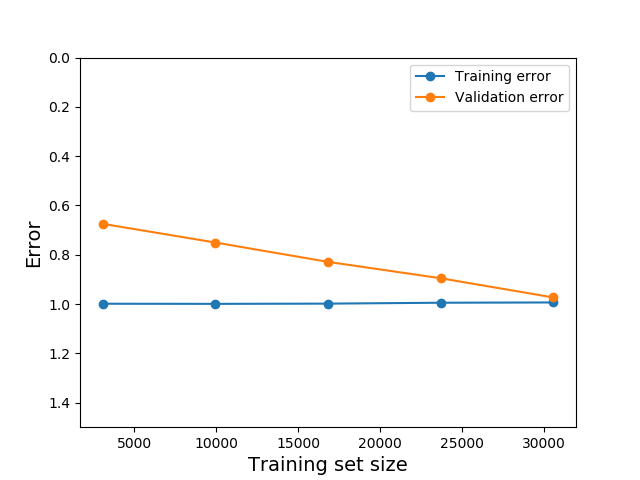
\includegraphics[width=1\linewidth]{../../models/training/simulator_rf_tuned_large_curves} 

}

\caption[Simulator Model Learning Curves]{Simulator Model Learning Curves}\label{fig:simulator_lc}
\end{figure}
\end{Schunk}

\hypertarget{lender-evaluator-1}{%
\subsection{Lender Evaluator}\label{lender-evaluator-1}}

Without further due let's apply the same methodology to select
\emph{Lender Evaluator} classifier.

\hypertarget{svm-1}{%
\paragraph{SVM}\label{svm-1}}

\begin{verbatim}
          precision    recall  f1-score   support

       1       0.98      0.96      0.97      4053
       2       0.93      0.94      0.94      3249
       3       0.88      0.93      0.90      1272
       4       0.81      0.83      0.82       209
       5       0.75      0.66      0.70        32

micro avg      0.94      0.94      0.94      8815
macro avg      0.87      0.86      0.87      8815
weighted avg   0.94      0.94      0.94      8815

Overall algorithm accuracy: 0.9441
\end{verbatim}

\hypertarget{random-forest-1}{%
\paragraph{Random Forest}\label{random-forest-1}}

\begin{verbatim}
          precision    recall  f1-score   support

       1       0.99      0.98      0.99      4038
       2       0.97      0.98      0.97      3289
       3       0.95      0.95      0.95      1261
       4       0.89      0.82      0.85       197
       5       0.89      0.53      0.67        30

micro avg      0.97      0.97      0.97      8815
macro avg      0.94      0.85      0.89      8815
weighted avg   0.97      0.97      0.97      8815

Overall algorithm accuracy: 0.972
\end{verbatim}

\hypertarget{gradient-boosting-1}{%
\paragraph{Gradient Boosting}\label{gradient-boosting-1}}

\begin{verbatim}
          precision    recall  f1-score   support

       1       0.99      0.95      0.97      4066
       2       0.92      0.92      0.92      3261
       3       0.81      0.87      0.84      1218
       4       0.67      0.86      0.75       235
       5       0.68      0.80      0.74        35

micro avg      0.93      0.93      0.93      8815
macro avg      0.81      0.88      0.84      8815
weighted avg   0.93      0.93      0.93      8815

Overall algorithm accuracy: 0.925
\end{verbatim}

\hypertarget{the-best-lender-evaluator-model}{%
\subsubsection{The Best Lender Evaluator
Model}\label{the-best-lender-evaluator-model}}

Again the \textbf{Random Forest} algorithm proved to be the most
accurate. Though it does not identify category 5 observations as well as
the other two algorithm we hope that the input data dimentionality
increase and the hyper-parameter tuning will fix the problem.

\begin{longtable}[]{@{}llll@{}}
\toprule
Category & \textbf{RF f1-score} & SVM f1-score & GB
f1-score\tabularnewline
\midrule
\endhead
1 & \textbf{0.99} & 0.97 & 0.97\tabularnewline
2 & \textbf{0.97} & 0.94 & 0.92\tabularnewline
3 & \textbf{0.95} & 0.90 & 0.84\tabularnewline
4 & \textbf{0.85} & 0.82 & 0.75\tabularnewline
5 & \textbf{0.67} & 0.70 & 0.74\tabularnewline
Accuracy & \textbf{0.972} & 0.9441 & 0.925\tabularnewline
\bottomrule
\end{longtable}

\hypertarget{dimensionality-change-1}{%
\subsubsection{Dimensionality Change}\label{dimensionality-change-1}}

Let's evaluate how the number of features affect the accuracy of the
model. Just like in the case of the simulator model we begin with the
smaller feature set, namely seven.

Top seven features:

\begin{longtable}[]{@{}ll@{}}
\toprule
Num & Feature\tabularnewline
\midrule
\endhead
24 & Do you receive your money back in time?\tabularnewline
26 & What's the most common use of the money you lend?\tabularnewline
22 & Do you include either interest or a lending fee when you
lend?\tabularnewline
18 & Over the past 3 months, how many times have you lent someone
money?\tabularnewline
20 & Who did you lend money to in the past 3 months?\tabularnewline
23 & Do you request guarantees when you lend?\tabularnewline
19 & On average how much do you lend in general?\tabularnewline
\bottomrule
\end{longtable}

Model Performance:

\begin{verbatim}
      precision    recall  f1-score   support

       1       0.99      0.97      0.98      4005
       2       0.96      0.95      0.95      3330
       3       0.89      0.95      0.92      1252
       4       0.84      0.92      0.88       205
       5       0.84      0.70      0.76        23

micro avg      0.96      0.96      0.96      8815
macro avg      0.90      0.90      0.90      8815
weighted avg   0.96      0.96      0.96      8815 

Overall algorithm accuracy: 0.9585    
\end{verbatim}

Surprisingly the dimentionality reduction resulted in better model
performance!

Top ten features:

\begin{longtable}[]{@{}ll@{}}
\toprule
\begin{minipage}[b]{0.05\columnwidth}\raggedright
Num\strut
\end{minipage} & \begin{minipage}[b]{0.89\columnwidth}\raggedright
Feature\strut
\end{minipage}\tabularnewline
\midrule
\endhead
\begin{minipage}[t]{0.05\columnwidth}\raggedright
24\strut
\end{minipage} & \begin{minipage}[t]{0.89\columnwidth}\raggedright
Do you receive your money back in time?\strut
\end{minipage}\tabularnewline
\begin{minipage}[t]{0.05\columnwidth}\raggedright
18\strut
\end{minipage} & \begin{minipage}[t]{0.89\columnwidth}\raggedright
Over the past 3 months, how many times have you lent someone
money?\strut
\end{minipage}\tabularnewline
\begin{minipage}[t]{0.05\columnwidth}\raggedright
22\strut
\end{minipage} & \begin{minipage}[t]{0.89\columnwidth}\raggedright
Do you include either interest or a lending fee when you lend?\strut
\end{minipage}\tabularnewline
\begin{minipage}[t]{0.05\columnwidth}\raggedright
23\strut
\end{minipage} & \begin{minipage}[t]{0.89\columnwidth}\raggedright
Do you request guarantees when you lend?\strut
\end{minipage}\tabularnewline
\begin{minipage}[t]{0.05\columnwidth}\raggedright
20\strut
\end{minipage} & \begin{minipage}[t]{0.89\columnwidth}\raggedright
Who did you lend money to in the past 3 months?\strut
\end{minipage}\tabularnewline
\begin{minipage}[t]{0.05\columnwidth}\raggedright
26\strut
\end{minipage} & \begin{minipage}[t]{0.89\columnwidth}\raggedright
What's the most common use of the money you lend?\strut
\end{minipage}\tabularnewline
\begin{minipage}[t]{0.05\columnwidth}\raggedright
19\strut
\end{minipage} & \begin{minipage}[t]{0.89\columnwidth}\raggedright
On average how much do you lend in general?\strut
\end{minipage}\tabularnewline
\begin{minipage}[t]{0.05\columnwidth}\raggedright
25\strut
\end{minipage} & \begin{minipage}[t]{0.89\columnwidth}\raggedright
Assuming that you have lent money at least ten times, how often would
you get your money repaid?\strut
\end{minipage}\tabularnewline
\begin{minipage}[t]{0.05\columnwidth}\raggedright
16\strut
\end{minipage} & \begin{minipage}[t]{0.89\columnwidth}\raggedright
Country\strut
\end{minipage}\tabularnewline
\begin{minipage}[t]{0.05\columnwidth}\raggedright
21\strut
\end{minipage} & \begin{minipage}[t]{0.89\columnwidth}\raggedright
When you lend money, when do you usually expect to get it repaid?\strut
\end{minipage}\tabularnewline
\bottomrule
\end{longtable}

Model Performance:

\begin{verbatim}
          precision    recall  f1-score   support

       1       0.99      0.99      0.99      4058
       2       0.97      0.98      0.97      3216
       3       0.94      0.96      0.95      1273
       4       0.92      0.85      0.88       229
       5       0.97      0.74      0.84        39

micro avg      0.98      0.98      0.98      8815
macro avg      0.96      0.90      0.93      8815
weighted avg   0.98      0.98      0.98      8815

Overall algorithm accuracy: 0.975
\end{verbatim}

The dimentionality increase yields the best performance. The category 5
identification has been improved the most. The top ten feature set is an
ultimate winner.

\begin{longtable}[]{@{}lllll@{}}
\toprule
Category & 7 Features** & 9 Features (base-line) & \textbf{10 Features}
& Gain (\%)\tabularnewline
\midrule
\endhead
1 & 0.98 & 0.99 & \textbf{0.99} & 0\tabularnewline
2 & 0.95 & 0.97 & \textbf{0.97} & 0\tabularnewline
3 & 0.92 & 0.95 & \textbf{0.95} & 0\tabularnewline
4 & 0.88 & 0.85 & \textbf{0.88} & 3\tabularnewline
5 & 0.76 & 0.67 & \textbf{0.84} & 17\tabularnewline
\bottomrule
\end{longtable}

\hypertarget{hyper-parameter-tuning-1}{%
\subsubsection{Hyper-parameter Tuning}\label{hyper-parameter-tuning-1}}

Though the selected model demonstrates quite spectacular accuracy we
would want to improve the identification of the category \# 5. We are
going to apply Grid Search algorithm again trying to find the optimal
hyper-parameters.

Parameter grid:

\begin{longtable}[]{@{}ll@{}}
\toprule
Parameter & Values\tabularnewline
\midrule
\endhead
Number of Estimators & 200, 300, 400\tabularnewline
Minimum Sample Split & 5, 10, 20, 30, 40\tabularnewline
Maximum Features & `auto', `sqrt'\tabularnewline
Bootstrap: & True, False\tabularnewline
\bottomrule
\end{longtable}

The hyper-parameter tuning has demonstrated similar to the default
parameter performance.

\hypertarget{final-evaluator-model-stats}{%
\subsubsection{Final Evaluator Model
Stats}\label{final-evaluator-model-stats}}

\begin{itemize}
\tightlist
\item
  Number of features: \textbf{10}
\item
  Overall algorithm accuracy: \textbf{0.9756}
\end{itemize}

\begin{Schunk}
\begin{figure}[H]

{\centering 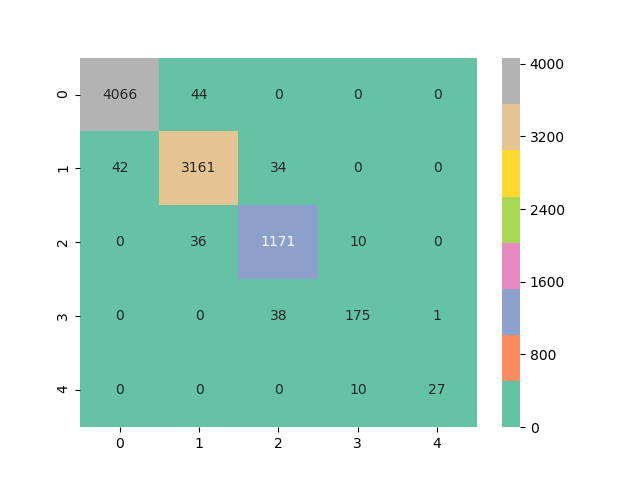
\includegraphics[width=1\linewidth]{../../models/training/evaluator_rf_tuned_large_matrix} 

}

\caption[Evaluator Model Confusion Matrix]{Evaluator Model Confusion Matrix}\label{fig:evaluator_cm}
\end{figure}
\end{Schunk}

\begin{verbatim}
       precision    recall  f1-score   support

       1       0.99      0.99      0.99      4110
       2       0.98      0.98      0.98      3237
       3       0.94      0.96      0.95      1217
       4       0.90      0.82      0.86       214
       5       0.96      0.73      0.83        37

micro avg      0.98      0.98      0.98      8815
macro avg      0.95      0.90      0.92      8815
weighted avg   0.98      0.98      0.98      8815
\end{verbatim}

Lastly we are going to review the model learning and validation curves.
Figure \ref{fig:evaluator_lc} is very similar to the simulator model
training and validation curves. The validation error curve does exhibit
interesting behavior. It is practically flat when the training set size
seats between 17000 and 25000. Then the validation curve converges with
training set curve. As we stated earlier the category \#4 and especially
\#5 were scarcely populated. Though we upsampled the categories we think
that the data lucks the variance. Probably if we collect more category 4
and 5 observations and apply enriched data set for model training the
model would perform better.

\begin{Schunk}
\begin{figure}[H]

{\centering 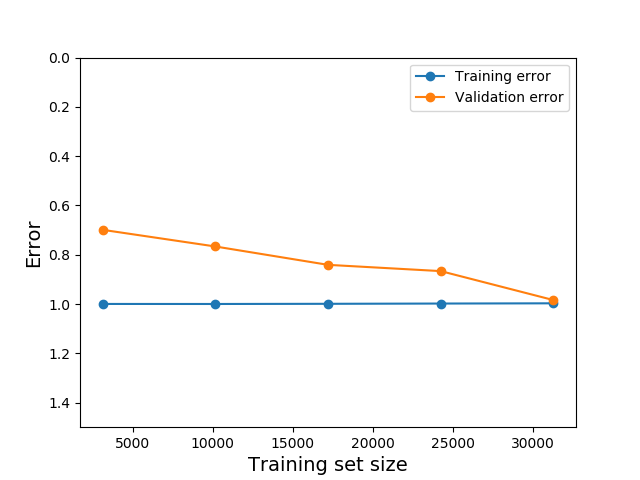
\includegraphics[width=0.9\linewidth]{../../models/training/evaluator_rf_tuned_large_curves} 

}

\caption[Eval Model Learning Curves]{Eval Model Learning Curves}\label{fig:evaluator_lc}
\end{figure}
\end{Schunk}

\hypertarget{model-deployment}{%
\section{Model Deployment}\label{model-deployment}}

The simulator and evaluator models were deserialized and persisted as
the pickle files. The model images were deployed to Flask Web
Application server and exposed as RESTful Web services.

\hypertarget{architecture}{%
\subsection{Architecture}\label{architecture}}

The following is the high-level description of the deployment
architecture:

\begin{enumerate}
\def\labelenumi{\arabic{enumi}.}
\tightlist
\item
  The front-end is a browser-based application developed using
  JavaScript, HTML/CSS and Angular framework. It utilized Restful API to
  communicate with the back-end.
\item
  The front-end Web application is packaged as a docker image and
  deployed in AWS EC2 instance.
\item
  The back-end is developed in Python employing various Python
  scientific libraries
\item
  The back-end code is hosted in Flask Web application server, which
  exposes two end-points - one for each model.
\item
  Flask Web Application is deployed in separate AWS EC2 instance
  utilizing the docker technology.
\item
  JSON Ajax POST request over HTTP is the exchange protocol between the
  tiers.
\end{enumerate}

\begin{Schunk}
\begin{figure}[H]

{\centering 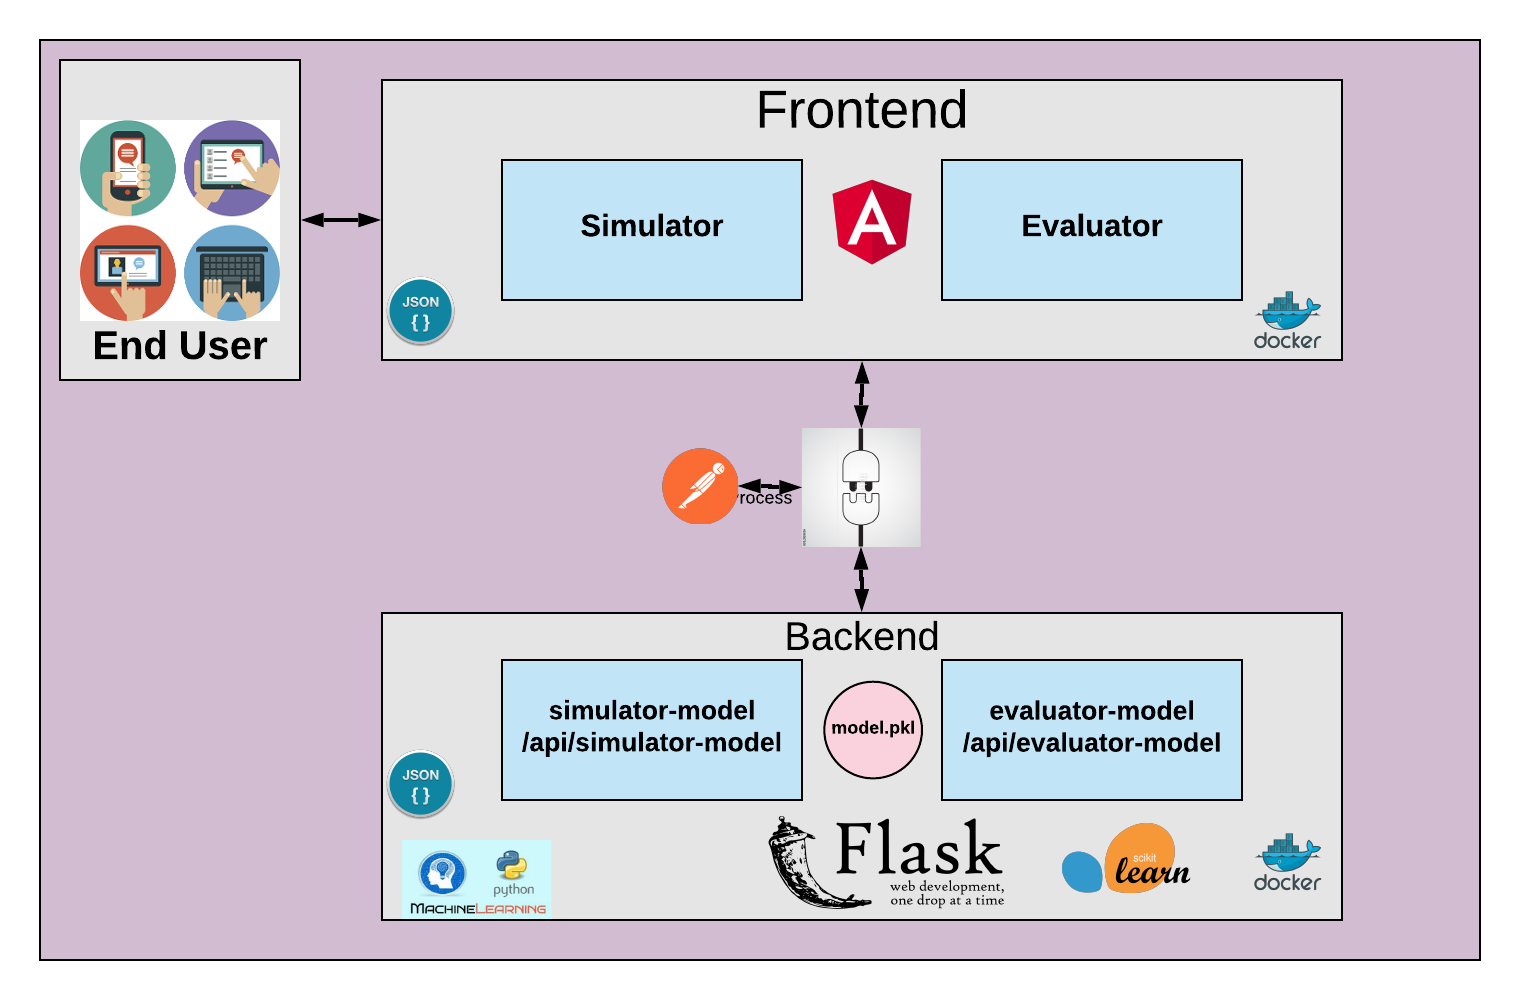
\includegraphics[width=1.15\linewidth]{../../artifacts/architecture} 

}

\caption[Deployment Architecture]{Deployment Architecture}\label{fig:arch}
\end{figure}
\end{Schunk}

\hypertarget{docker}{%
\subsection{Docker}\label{docker}}

We opted to utilize \textbf{Docker} technology to simplify the
deployment of the application to the cloud environment. Once the docker
images are generated, same gets published within docker registry or with
AWS ECR. The images can be pulled from the image repository for
deployment in AWS EC2 or local server as per needs.

\begin{Schunk}
\begin{figure}[H]

{\centering 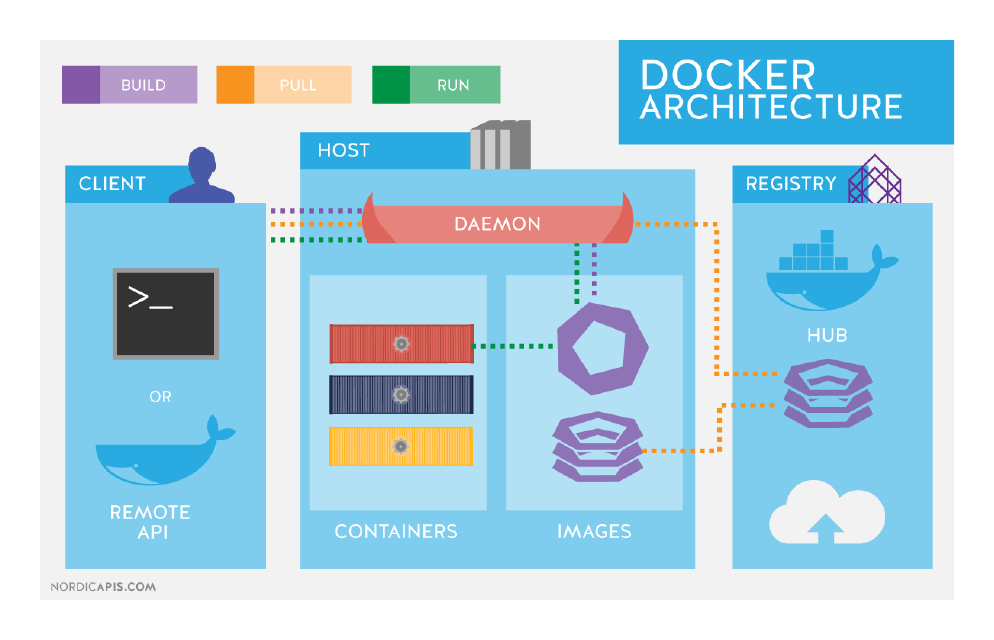
\includegraphics[width=1.15\linewidth]{../../artifacts/docker} 

}

\caption[Docker Image,Container and Registry]{Docker Image,Container and Registry}\label{fig:di}
\end{figure}
\end{Schunk}

\hypertarget{conclusion}{%
\section{Conclusion}\label{conclusion}}

We started this project with learning the business of KASI Insight - our
partner. We explored the company data, understood its challenges and
objectives. After gaining good feel about the company and its business
we suggested a few concepts that we believed would allow our business
partner to extend its offering. The concepts employed Machine-Learning
techniques. Working closely with KASI Insight team we developed a
methodology that allowed us to apply KASI Insight data to train the ML
models. As a result of this close collaboration we came up with a
project proposal that met the objectives of our business partner and
allowed us to hone our ML skills. We promised to:

\begin{itemize}
\tightlist
\item
  Develop Lending Environment Simulator model.
\item
  Train Lender Evaluator model.
\item
  Deliver key-turn solution that would include:

  \begin{itemize}
  \tightlist
  \item
    an on-line service that provides access to the model algorithms.
  \item
    a Web-based client that would demonstrate the models in action.
  \item
    a Docker image that would include all software tiers and be used for
    easy deployment of the system to cloud environment.
  \end{itemize}
\end{itemize}

We can proudly conclude that we have achieved all these goals.

\bibliography{RJreferences}

\hypertarget{note-from-the-authors}{%
\section{Note from the Authors}\label{note-from-the-authors}}

This file was generated using
\href{https://github.com/rstudio/rticles}{\emph{The R Journal} style
article template}, additional information on how to prepare articles for
submission is here -
\href{https://journal.r-project.org/share/author-guide.pdf}{Instructions
for Authors}. The article itself is an executable R Markdown file that
could be
\href{https://github.com/ivbsoftware/big-data-final-2/blob/master/docs/R_Journal/big-data-final-2/}{downloaded
from Github} with all the necessary artifacts.


\address{%
Vadim Spirkov\\
York University School of Continuing Studies\\
\\
}


\address{%
Murlidhar Loka\\
York University School of Continuing Studies\\
\\
}


